\chapter{Learning graph-based analysis heuristics without features~\footnote{The contents of this chapter are based on our previous work presented at \emph{OOPSLA 2020: ACM Conference on Object-Oriented Programming, Systems, Languages, and Applications}~\cite{Graphick20}}}\label{sec:Graphick}


This chapter presents a new technique for automatically learning graph-based heuristics for pointer analysis.
Past research has shown that exploiting the program's graph structure is a promising way of developing cost-effective analysis heuristics, promoting the recent trend of ``graph-based heuristics'' that work on the graph representations of programs obtained from a  pre-analysis. 
Although promising, manually developing such heuristics remains challenging, requiring a great deal of expertise and laborious effort.
In this chapter, we aim to reduce this burden by learning graph-based heuristics automatically, in particular without hand-crafted application-specific features. To do so, we present a feature language to describe graph structures and an algorithm for learning analysis heuristics within the language.
We implemented~\ourtool~on top of \Doop~and used it to learn graph-based heuristics for object sensitivity and heap abstraction.
The evaluation results show that our approach is general and can generate high-quality heuristics. For both instances,
the learned heuristics are as competitive as the existing state-of-the-art heuristics designed manually by analysis experts.







\tikzstyle{block} = [rectangle,   text width=3.5em, text
centered, rounded corners, minimum height=3em]



\tikzstyle{myCircle} = [circle,thick,draw=black!75   text width=3.5em, text
centered, minimum height=3em]


\tikzstyle{block2} = [rectangle,   text width=2em, text
centered, rounded corners, minimum height=3em]

\tikzstyle{line} = [draw, -latex']
\tikzstyle{onlyText} = [text width =5em, text centered]
\tikzstyle{smallOnlyText} = [text width =15em, text centered]
\tikzstyle{None} = [text width =0em, text centered]
\tikzstyle{longText} = [text width = 20em, text centered]

%\setcopyright{rightsretained}


\tikzstyle{block4} =
[rectangle, draw, fill=white, text width=10.5em, text centered, rounded
corners, minimum height=2.3em]
\tikzstyle{block3} =
[rectangle, draw, fill=white, text width=9em, text centered, rounded
corners, minimum height=2.3em] \tikzstyle{line} = [draw, -latex']


\tikzstyle{blocks} = [rectangle, draw, fill=white, text width=0.7cm, text
centered,  text width=4em, rounded corners, minimum height=0.5cm]


% !TEX root = ./paper.tex

\section{Introduction}
\iffalse
Pointer analysis is a fundamental program analysis technique that serves as a
key component of various software engineering tools.  The goal of
pointer analysis is to statically and conservatively estimate heap objects that
pointer variables may refer to at runtime.  The pointer
information is essential for virtually all kinds of program analysis tools, including bug
detectors~\cite{Naik2006,NaikPSG09,Blackshear2015,Sui2014,Livshits2003},
security analyzers~\cite{Avots2005,Arzt2014,Tripp2009,Yan2017,Grech17},
program verifiers~\cite{Fink2008}, symbolic executors~\cite{Kapus2019}, and program
repair tools~\cite{memfix,Gao2015,vfix2019,saver2020}. The success of these tools depends eventually on the precision and scalability of the underlying pointer analysis algorithm.
\fi

Developing a fast and precise pointer analysis requires coming up with good analysis heuristics.
For example, context sensitivity is critical for accurately analyzing object-oriented programs as it distinguishes method's local variables and objects in different calling contexts~\cite{Smaragdakis2015}. In reality, however, it is too expensive to apply deep context sensitivity (e.g. 2-object-sensitivity) to all methods in a nontrivial program.
Therefore practical pointer analysis applies context sensitivity selectively using a context abstraction heuristic that determines the  amount of context sensitivity that each method should receive~\cite{Smaragdakis2014,JeJeChOh17,Li2018a,Lu2019}.
Similarly, the performance of pointer analysis depends heavily on how heap objects are represented~\cite{DBLP:journals/csur/KanvarK16}.
Pointer analysis usually employs allocation-site-based heap abstraction, which models heap objects with their allocation sites.
However, because uniformly applying it to all heap objects is costly, a heap abstraction heuristic can be used to apply it selectively and otherwise use a less precise scheme such as type-based abstraction~\cite{Tan2017}.


\myparagraph{Trend: Graph-based Heuristics}

A recent trend in state-of-the-art pointer analyses is use of graph-based analysis heuristics~\cite{Li2018a,Li2018b,Tan2017,TanLX16,Lu2019,JeOh22}.
These graph-based heuristics commonly work in the following two steps:
(1) they first use a cheap pre-analysis to construct a graph representation of the input program and
(2) they reason about the graph structure to produce a program-specific policy for the main analysis.

For example,
\cite{TanLX16} presented \Bean, which first runs a context-insensitive
pre-analysis to generate the object allocation graph (OAG)
and infers from it a policy  for improving the precision of $k$-object-sensitive analysis.
\cite{Li2018b} proposed \Scaler, which also uses a context-insensitive pre-analysis to derive the object allocation graph and analyzes its structure to identify method calls that are likely to blow up the analysis cost during the 2-object-sensitive analysis.
%With this information, \Scaler~applies 2-object sensitivity selectively in the main analysis.
\cite{Li2018a} presented \Zipper, another graph-based heuristic for context-sensitive analysis.
\Zipper~uses a pre-analysis to generate a so-called precision flow graph (PFG)
and identifies precision-critical method calls that may lose precision significantly if context insensitivity is used.
 \cite{Lu2019} presented
a graph-based heuristic, called \Eagle,~that uses a CFL-reachability-based pre-analysis to find out variables and objects that need
context sensitivity in the main analysis.
\cite{Tan2017} developed \Mahjong, a graph-based heap
abstraction heuristic that first runs a cheap pre-analysis to derive a field points-to graph (FPG) and decides when to merge and differentiate heap objects based on the structure of the points-to graph.

%All of the
%graph-based heuristics above are manually designed with a variety of
%insights by pointer analysis experts.
%
%
%, which reveals the
%contexts to be produced in
%$k$-object-sensitivity~\cite{Milanova2002,Milanova2005,Smaragdakis2011}.
%Using the derived graph, it produces analysis strategies that
%determine the appropriate heap contexts for each object, which
%improves the precision of the main analysis (e.g.,
%2-object-sensitivity).  In like manner, \cite{Li2018b} proposes a
%context-sensitivity heuristic \Scaler~which employs the same
%pre-analysis and the type of graph as mentioned above.  From an
%object-allocation-graph, it figures out the method calls which would
%likely blow up the analysis costs when applying
%$2$-object-sensitivity; with this information, it applies cheap
%alternative contexts for them in the main analysis.  \cite{Li2018a}
%introduces another graph-based context-sensitivity heuristic \Zipper.
%It uses a precision-flow-graph, an extended version of an
%object-flow-graph~\cite{Tonella05}, which can predict the precision
%loss occurred when we apply coarse context-sensitivity.  To obtain
%this graph,~\cite{Li2018a} performs context insensitive analysis as a
%pre-analysis and then figures out precision-critical method calls
%based on the information in the graph.  \cite{Tan2017} designs heap
%abstraction heuristic \Mahjong~from field-points-to-graphs, where the
%nodes are the heap objects.  Field-points-to-graphs represent each
%object's field as a graph of which nodes are connected when a field of
%an object points-to the other objects.  \Mahjong~runs a cheap
%pre-analysis to obtain this graph and merges objects when their
%successor objects have the same type.  \cite{Lu2019} presents
%lightweight pre-analysis corresponding to CFL-reachability formulation
%of $k$-object-sensitivity to find out variables and objects that need
%to be analyzed context-sensitively in the main analysis.  All of the
%graph-based heuristics above are manually designed with a variety of
%insights by pointer analysis experts.

\myparagraph{This Work}

we aim to advance this line of research by automating the process of creating graph-based analysis heuristics for pointer analysis.
While all of the existing graph-based heuristics have been designed manually by analysis experts,
our technique generates such heuristics automatically from a given graph without any human effort, significantly increasing  applicability and accessibility of the emerging and promising approach in pointer analysis.

We achieve this goal by developing (1) a feature language for describing graph structures and (2) an algorithm for learning analysis heuristics in terms of the sentences of the language.
We first present a language for describing structural features of nodes in a graph.
This feature description language is simple and general, allowing it to be reused for various analysis instances (e.g. object sensitivity and heap abstraction).
Second, we present a learning
algorithm that takes training programs (and their graph representations) and produces graph-based heuristics by
automatically discovering features appropriate for the given analysis task.
Compared to prior data-driven static analysis techniques~\cite{JeJeChOh17,JeJeOh18,Singh2018cav,He20pldi},
a salient characteristic of our technique is that it does not require pre-designed, application-specific features; instead, it uses a feature language to generate a proper set of features during the learning process. By contrast, existing learning-based techniques for static analysis need a different set of hand-tuned features for each analysis task.

% The algorithm first figures out
%performance-critical nodes in the graph
%produced by the pre-analysis of the training programs, and it
%formulates the nodes as features using the feature language.  The
%generated features describe the performance-critical nodes of graph,
%which constitute analysis heuristics for the main analysis.


The evaluation results show that our technique is effective and general;
it can automatically produce competitive heuristics for two different analysis instances.
We implemented our approach on top of the \Doop~pointer
analysis framework for Java~\cite{BravenboerS09}.
We used our approach to produce
a object-sensitivity heuristic from the object allocation graph on
which the state-of-the-art object-sensitivity heuristic
\Scaler~\cite{Li2018b} was developed.
Additionally, we learned a heap
abstraction heuristic from the field points-to graph, which is
 used in the state-of-the-art heap abstraction heuristic
\Mahjong~\cite{Tan2017}.  For both instances, our approach
successfully generated high-quality heuristics that are as competitive as
\Scaler~and \Mahjong~in terms of the precision and scalability of the main analysis.
In particular, the generated heuristic by our framework successfully
analyzes large programs which the state-of-the-art heap abstraction
heuristic, \Mahjong, cannot handle within a time budget.

%perform as cost-effectively as the state-of-the-art techniques do.



\myparagraph{Contributions}
In summary, this paper makes the following contributions:
\begin{itemize}
\item We present~\ourtool, a new technique for automatically learning graph-based heuristics for pointer analysis.
Key technical contributions include a feature description language and a learning algorithm, which allow our approach to be generally used for different analysis instances without manually designing application-specific features.
%design a new feature language for describing properties of
%  nodes in graphs. The feature language is simple and general; it can
%  be applied to any graphs.
%\item We develop a learning algorithm that automatically generates
%  features as analysis heuristics. It includes an effective algorithm
%  to find out performance-critical program components that the
%  algorithm is an advance one from~\cite{Liang2011learning}.
\item We demonstrate the effectiveness and generality of our technique in comparison with state-of-the-art heuristics for object sensitivity and heap abstraction.

%
%evaluate our approach for two important analysis tasks, namely context sensitivity and heap abstraction, using real-world pointer analysis algorithms and benchmarks.
%heuristic instances and graphs.
%We show that the learned heuristics are cost-effective.
\end{itemize}



%%% Local Variables:
%%% mode: latex
%%% TeX-master: "paper"
%%% End:































%\newpage
\section{Motivating Example}
\label{sec:overview}

In this section, we motivate our idea of context tunneling with a simple example. We
explain our technique in the context of call-site-sensitivity, but it
is also applicable
to other flavors of context-sensitivity too, such as object-sensitivity and
type-sensitivity. The general description is presented in
Section~\ref{sec:tunneling}.

\myparagraph{Example Code}

Suppose that we analyze the example Java code in
Fig.~\ref{fig:overview}(a) using a $k$-call-site-sensitive points-to
analysis~\cite{Smaragdakis2015}.  The example code has three class
definitions, namely \texttt{A}, \texttt{B}, and \texttt{C}.  Classes
\texttt{A} and \texttt{B} are empty and class \texttt{C} has two
methods: \texttt{id} and \texttt{main}.  Method \texttt{id} is
essentially an identity function on the first argument, which takes an
object \texttt{v} and an integer \texttt{i}, and returns the same
object after making recursive calls until \texttt{i} becomes 0. In
\texttt{main}, \texttt{id} is invoked twice with different
objects. Both method invocations share the same argument \texttt{i}
that comes from the external environment (i.e. user input).  The goal
of the points-to analysis is to prove the safety of two type casts at
lines 8 and 9.

\begin{figure}
\centering
\begin{subfigure}[b]{.45\columnwidth}
\begin{lstlisting}
class A {} class B {}
class C {
  static Object id (Object v, int i){
      return i >= 0 ? id(v, i-1) : v;
  }
  public static void main (){
    int i = input();
    A a = (A) id(new A(), i);	//Query 1
    B b = (B) id(new B(), i);	//Query 2
  }
}
\end{lstlisting}
\caption{Example code}
\label{fig:overview:code}
\end{subfigure}
\quad
\begin{subfigure}[b]{.45\columnwidth}

%%% k-CFA
\begin{center}
\resizebox{\columnwidth}{!}{
\begin{tikzpicture}
    \node [block] (main) {{\tt main} \\ $[\cdot]$};
    \node [block, above right=0cm and 0.4cm of main] (id1) {{\tt id}\\$[8]$};
    \node [block, below right=0cm and 0.4cm of main] (id2) {{\tt id}\\$[9]$};
    \node [block, right=0.4cm of id1] (id3) {{\tt id} \\$[8,4]$};
    \node [block, right=0.4cm of id2] (id4) {{\tt id} \\$[9,4]$};
    \node [block2, right=0.4cm of id3] (id5) {{\tt id}\\$[\underbrace{8,4,\cdots,4}_k]$};
    \node [block2, right=0.4cm of id4] (id6) {{\tt id}\\$[\underbrace{9,4,\cdots,4}_k]$};
    \node [block2, below right=0cm and 0.4cm of id5] (id7) {{\tt id} \\$[\underbrace{4,\cdots,4}_{k}]$};

    \path [line] (main) -- (id1);
    \path [line] (main) -- (id2);
    \path [line] (id1) -- (id3);
    \path [line] (id2) -- (id4);
    \path [line, dashed] (id3) -- (id5);
    \path [line, dashed] (id4) -- (id6);
    \path [line] (id5) -- (id7);
    \path [line] (id6) -- (id7);
    \path [line] (id7) edge[loop above] ();
\end{tikzpicture}
}
\end{center}


%%% 2-CFA
% \begin{center}
% \resizebox{\columnwidth}{!}{
% \begin{tikzpicture}
%     \node [block] (main) {{\tt main} \\ $[\cdot]$};
%     \node [block, above right=0cm and 0.4cm of main] (id1) {{\tt id}\\$[8]$};
%     \node [block, below right=0cm and 0.4cm of main] (id2) {{\tt id}\\$[9]$};
%     \node [block, right=0.4cm of id1] (id3) {{\tt id} \\$[8,4]$};
%     \node [block, right=0.4cm of id2] (id4) {{\tt id} \\$[9,4]$};
%     \node [block, below right=0cm and 0.4cm of id3] (id7) {{\tt id} \\$[4,4]$};

%     \path [line] (main) -- (id1);
%     \path [line] (main) -- (id2);
%     \path [line] (id1) -- (id3);
%     \path [line] (id2) -- (id4);
%     \path [line] (id3) -- (id7);
%     \path [line] (id4) -- (id7);
%     \path [line] (id7) edge[loop above] ();
% \end{tikzpicture}
% }
% \end{center}
\caption{Call-graph by $k$-CFA}

\vspace{2ex}

\begin{center}
\resizebox{0.5\columnwidth}{!}{
\begin{tikzpicture}
    \node [block] (main) {{\tt main}\\$[\cdot]$};
    \node [block, above right=0cm and 0.5cm of main] (id1) {{\tt id}\\$[8]$};
    \node [block, below right=0cm and 0.5cm of main] (id2) {{\tt id}\\ $[9]$};

    \path [line] (main) -- (id1);
    \path [line] (main) -- (id2);

    \path [line] (id1) edge[loop right] ();
    \path [line] (id2) edge[loop right] ();
\end{tikzpicture}
}
\end{center}
\caption{Call-graph by 1-CFA with tunneling}
\end{subfigure}\qquad
\caption{Example and call-graphs constructed by the conventional 2-call-site sensitivity (2-CFA) and our 1-call-site-sensitivity with tunneling}
\label{fig:overview}
\end{figure}

\myparagraph{Conventional Context-Sensitive Analysis}


The conventional $k$-call-site-sensitive analysis fails to prove the queries no matter what $k$ value is used.
Because the value of \texttt{i} can be any integer, the following set $K_{\infty}$ of infinite number of call-strings can be generated for method \texttt{id} at runtime:
\[
K_{\infty} = \myset{[8], [9], [8,4], [9,4], [8,4,4], [9,4,4], [8,4,4,4], [9,4,4,4], \dots}
\]
where, for example, $[8,4]$ denotes the context that method \texttt{id} was called along the sequence of call-sites 8 and 4. The $k$-call-site-sensitive analysis approximates the call-strings in $K_{\infty}$ by their suffixes of length up to $k$. For example, when $k=2$, the analysis uses the following set $K_2$ of abstract contexts:
\[
K_2 = \myset{[8], [9], [8,4], [9,4], [4,4]}
\]
where an infinite number of contexts, $\myset{[8,4,4], [9,4,4], [8,4,4,4], [9,4,4,4],\dots}$, in $K_{\infty}$ are approximated by their common suffix $[4,4]$. The analysis analyzes the method \texttt{id} separately for each context in $K_2$. % producing the call-graph in Fig.~\ref{fig:overview}(b).
Although this approximation ensures termination, the analysis is now unable to differentiate the two separate calls to \texttt{id} at lines 8 and 9, causing the argument {\tt v} of {\tt id} to point to both objects {\tt A} and {\tt B} at the same time when the context is $[4,4]$. Thus, both objects get returned to both queries simultaneously, making the analysis fail to prove their cast safety.
Note that the analysis fails to prove the queries for any $k$ values, because all the context strings longer than $k$ are eventually
merged into a single context $[\underbrace{4,\dots,4}_{k}]$ (see Fig.~\ref{fig:overview}(b)).


\myparagraph{The Idea of Context Tunneling}

With context tunneling, however, even $1$-call-site sensitive analysis
becomes to prove the queries.
% Our idea to improve the analysis is to identify and maintain important
% context elements only.
The main weakness of the conventional
$k$-context-sensitive analysis is that it blindly updates the context
of a method at every call-site, thereby allowing important context
elements for the method to be easily overwritten by less important
ones.  In the example, distinguishing the two call-sites
at lines 8 and 9 is essential to proving the queries. However, this
information is eventually lost by repeatedly appending the less
important call-site 4 to the context of {\tt id}
(Fig.~\ref{fig:overview}(b)).
Our technique aims to overcome this weakness by maintaining important
context elements only during analysis. For example, we exclude the
call-site 4 from the context strings generated for method {\tt id} and
thus approximate the set $K_{\infty}$ to the set $K_T$ of contexts:
\[
K_T = \myset{[8], [9]}.
\]
Here abstract contexts $[8]$ and $[9]$ in $K_{T}$ denote the sets of concrete contexts
$\myset{[8], [8,4], [8,4,4], \dots}$ and
$\myset{[9], [9,4], [9,4,4], \dots}$ in $K_{\infty}$, respectively. The resulting
context-sensitive analysis with $K_{T}$ is able to prove the queries as it differentiates the two calls
to {\tt id} at lines 8 and 9 completely, producing the call-graph in
Fig.~\ref{fig:overview}(c).

% With context tunneling, however, even $1$-call-site sensitive analysis
% is able to prove the queries.


This example shows that the idea of context tunneling is potentially
powerful; even $1$-context-sensitivity with
tunneling can be as precise as
$\infty$-context-sensitivity. The goal of this paper is to maximize
this tremendous, yet untapped, potential of the existing $k$-context-sensitive analysis.

\myparagraph{Challenge}

However, achieving effective context tunneling is
challenging. The effectiveness of the technique is very sensitive
to the choice of important context elements.  For example,
choosing the call-site 4, rather than call-sites 8 and 9, as important does not
work for the example program.  In the worst case, the analysis
precision degenerates into the context-insensitive case (e.g. when
selecting no context elements at all), becoming even inferior to the
ordinary
$k$-context-sensitive analysis.  As a result, coming up with a good
heuristic rule for choosing important context elements is nontrivial;
hand-crafting such a rule not only requires a huge amount of
engineering effort and domain knowledge but also likely fails to
maximize the potential of the technique.
% adaptable as a fixed heuristic rule tuned for a particular situation
% may not be effective for other programs, analyses, or queries.

%
\myparagraph{A Data-Driven Approach}


We address this challenge with a data-driven approach that
automatically learns a good tunneling heuristic from training data.
To do so, we first define a parameterized heuristic $\heuristic_\Pi$
(where $\Pi$ is a parameter). $\heuristic_\Pi$ takes a program and
returns a relation $\TunnelingRelation$ on methods such that
the relation contains a method pair $(m_1, m_2)$ if the calling
context of $m_1$ is more important than that
of $m_2$. Thus, if $(m_1, m_2) \in \TunnelingRelation$, the analysis
applies context tunneling for $m_2$; that is, $m_2$ inherits the context of
$m_1$ ignoring the current context element. For
the example program, $\heuristic_\Pi$ produces the
relation $\TunnelingRelation = \myset{({\tt id}, {\tt id})}$, which means that tunneling is applied to
{\tt id} when {\tt id} is called from itself. As a result, the
call-site 4, on which {\tt id} is called from {\tt id}, will not
be used as important context elements during analysis.  When {\tt main} calls
{\tt id}, however, the analysis updates the contexts as ordinary since
$({\tt main}, {\tt id}) \not\in \TunnelingRelation$.

The parameter $\Pi$ controls the behavior of the heuristic
$\heuristic_\Pi$.
Following the recent data-driven technique by~\citet{JeJeChOh17}, the
parameter $\Pi$ consists of boolean formulas over
atomic features on methods. We use two boolean formulas $\fprime$ and
$\fsecond$, which describe the sets of methods whose calling contexts
are important and unimportant, respectively.
For example, suppose we are given three atomic features
$\mba = \myset{a_1,a_2,a_3}$, where a feature $a_i : \mbox{Method} \to \myset{\true, \false}$ is a
predicate on methods (e.g. whether the return type of a method is
string, etc) and
assume that the methods {\tt main} and {\tt id} in the example
code have the features as follows:
\[
\begin{array}{llll}
&a_1({\tt main}) = \false, \quad &a_2 ({\tt main}) = \false, \quad &a_3({\tt main}) =
\true \\
&a_1({\tt id}) = \true, \quad &a_2({\tt id}) = \true,  \quad& a_3({\tt id}) = \false
\end{array}
% \mbox{features}({\tt main}) = \myset{a_3}, \qquad \mbox{features}({\tt
%   id}) = \myset{a_1, a_2}.
\]
Then, the following formulas $\fprime$ and $\fsecond$
\[
\fprime = a_1 \land \neg a_3, \qquad \fsecond = a_2 \land \neg a_3
\]
represent the sets of methods as follows:
\[
\db{\fprime} = \myset{{\tt id}}, \qquad \db{\fsecond}=\myset{{\tt id}}.
\]
Given $\Pi = \myset{\fprime, \fsecond}$, the heuristic
$\heuristic_\Pi$ produces the tunneling relation $\TunnelingRelation$
as follows:
\[
\TunnelingRelation = \myset{(m_1,m_2) \mid m_1 \in \db{\fprime} \vee m_2
  \in \db{\fsecond}}.
\]
That is, we apply tunneling if the caller context is important or the
callee context is unimportant.
Thus, the effectiveness of tunneling depends on $\Pi = \myset{\fprime,
  \fsecond}$ and it is the job of the learning algorithm to find
formulas $\fprime$ and $\fsecond$ such that the analysis with
$\heuristic_\Pi$ consistently performs well on a wide range of programs.

\myparagraph{Learning Context Tunneling Heuristics}
\begin{figure}
\begin{multicols}{2}
\begin{lstlisting}
Class A{} Class B{}
Class C{
	static Object id(Object v){
		return v;
	}
	static Object idrec(Object v, int i){
		return i >= 0 ? idrec(v, i-1) : v;
	}	
	static Object id1(Object v){
		return id(v);
	}
	static Object id2(Object v, int i){
		return idrec(v,i);
	}

	public static void main(){
		int i = input();
		A a1 = (A) id(new A());       //Q1
		B b1 = (b) id(new B());       //Q2
		A a2 = (A) id(new A());       //Q3
		B b2 = (b) id(new B());       //Q4
		
		A a3 = (A) id1(new A());      //Q5
		B b3 = (B) id1(new B());      //Q6
		
		A a4 = (A) id2(new A(), i);   //Q7
		B b4 = (B) id2(new B(), i);   //Q8
	}
}
\end{lstlisting}
\end{multicols}
\caption{Extended example code}
\label{fig:overview:new}
\end{figure}
We illustrate how our learning algorithm infers the tunneling relation, more specifically two Boolean formulas $\fprime$ and $\fsecond$. We extended previous example code to have three additional identity functions (i.e., \texttt{id1}, \texttt{id2}, and \texttt{idrec}) and more queries (i.e., Q1 -- Q8) as shown in Figure~\ref{fig:overview:new}. For simplicity, we consider the example code as sole training program, and suppose we are about to learn tunneling heuristic for $\onecallH$ using four atomic features $\afeatures=\myset{a, b, c, d}$. The goal of the learning algorithm is finding good heuristic parameter $\params=\langle \fprime, \fsecond \rangle$ that maximizes analysis precision (i.e., prove all queries) while keeping cost as small as conventional analysis.

Before we begin, we briefly explain a desirable context tunneling relation $\TunnelingRelation$ to prove eight queries Q1 -- Q8 in the example code with $\onecallHT$.
\begin{itemize}
\item {\bf Q1 -- Q4}: Applying conventional $\onecallH$ is enough to prove those queries. In terms of context tunneling, therefore, four {\tt id} invocations in {\tt main} (lines 18 -- 21) should generate context information as usual and hence the desirable tunneling relation $\TunnelingRelation$ shouldn't have $({\tt main}, {\tt id})$ relation in it.
\item {\bf Q5 and Q6}: Passing two {\tt id1} invocations' context to their descendants (i.e., {\tt id}) can prove those two queries because a call-site of {\tt id} (i.e., [10]) has less information gain. In other words, $\TunnelingRelation$ should have $({\tt id1}, {\tt id})$ relation. Note that this inclusion makes analysis to treat {\tt id} invocations differently with regard to their callers. Hence, invocations in line 18 -- 21 are analyzed in conventional way but one in line 10 gets context tunneling.
\item {\bf Q7 and Q8}: {\tt idrec} method calls should inherit context information from their callers in order to prove those two queries. In terms of context tunneling, $\TunnelingRelation$ should include $({\tt id2}, {\tt idrec})$ and $({\tt idrec}, {\tt idrec})$ relations.
\end{itemize}
All in all, $\onecallHT$ can prove all queries in the example under the desirable context tunneling relation $\TunnelingRelation$:
\[
\TunnelingRelation=\myset{({\tt id1}, {\tt id}), ({\tt id2}, {\tt idrec}), ({\tt idrec}, {\tt idrec})}
\]
Remaining of this subsection illustrates how our learning process infers two Boolean formulas $\fprime$ and $\fsecond$ to imply the desirable relations $\TunnelingRelation$.

\paragraph{Sketch of learning} Our learning algorithm begins with learning $\fsecond$, which means callee methods who should inherit context information from their callers instead of generating new ones. After that, our algorithm uses very same procedure to learn $\fprime$ to distinguish caller methods that should propagate their context information to descendants with regard to $\fsecond$. That means, we learn $\fprime$ such that, propagating context information from $m' \in \sem{\fprime}$ to its descendants increases precision even if one of descendant methods $m$ is meant to generate context information because $m \notin \sem{\fsecond}$.


\paragraph{Learning a Single Parameter $\fsecond$} Learning $\fsecond$ starts with setting baseline parameter $\params$ to $\langle \false, \false \rangle$, which means conventional analysis (i.e., $\onecallH$). Using the baseline parameter, our learning algorithm identifies a set of atomic features $W$ who has context tunneling potential. We say an atomic feature $a$ has potential if $\params_a=\langle \false, \fsecond=a \rangle$ makes analysis to prove queries that the baseline analysis can't. Suppose that each atomic feature means methods as follows:
\begin{equation} \label{eq:atoms}
\begin{aligned}
\sem{a}(P) & = & \myset{\texttt{id1}, \texttt{id2}, \texttt{idrec}} & \quad\quad & \sem{b}(P) & = & \myset{\texttt{id}, \texttt{id2}, \texttt{idrec}}\\
\sem{c}(P) & = & \myset{\texttt{id}, \texttt{id1}, \texttt{idrec}} & \quad\quad & \sem{d}(P) & = & \myset{\texttt{id}, \texttt{id1}, \texttt{id2}}
\end{aligned}
\end{equation}

Evaluating each atomic features including the baseline parameter gives following tunneling relations and precisions:
\begin{center}
% $\myset{(main, id), (main, id1), (main, id2), (id1, id), (id2, idrec), (idrec, idrec)}$
\begin{tabular}{c|c|c}
  \hline
  $\fsecond$ & Tunneling Relation $\TunnelingRelation$ & Proven queries\\
  \hline \hline
  $\false$ & $\emptyset$ & Q1, Q2, Q3, Q4 \\
  $a$ & $\myset{({\tt main}, {\tt id1}), ({\tt main}, {\tt id2}), ({\tt id2}, {\tt idrec}), ({\tt idrec}, {\tt idrec})}$ & Q1, Q2, Q3, Q4 \\
  $b$ & $\myset{({\tt main}, {\tt id}), ({\tt main}, {\tt id2}), ({\tt id1}, {\tt id}), ({\tt id2}, {\tt idrec}), ({\tt idrec}, {\tt idrec})}$ & \underline{Q5}, \underline{Q6} \\
  $c$ & $\myset{({\tt main}, {\tt id}), ({\tt main}, {\tt id1}), ({\tt id1}, {\tt id}), ({\tt id2}, {\tt idrec}), ({\tt idrec}, {\tt idrec})}$ & \underline{Q7}, \underline{Q8} \\
  $d$ & $\myset{({\tt main}, {\tt id}), ({\tt main}, {\tt id1}), ({\tt main}, {\tt id2}), ({\tt id1}, {\tt id})}$ & $\emptyset$ \\
  \hline
\end{tabular}
\end{center}
For example, evaluating $\fsecond = \myset{a}$ results same precision with the baseline. Method {\tt id}, which isn't belong to $\TunnelingRelation$, invocations generate context information hence four queries Q1 -- Q4 are provable. For the other queries, it fails to prove because important methods (i.e., {\tt id1} and {\tt id2}) are belong to $\TunnelingRelation$ hence they inherit context information from {\tt main}, which is less informative.

From the evaluation, our algorithm initializes workset $W$ with the features who proved queries except Q1 -- Q4, which are provable by the baseline parameter. We call them ``seed features''. The learning process ends after refining each seed feature in $W$:
\[
W=\myset{b, c}
\]

\paragraph{Refining Seed Feature} Than, our algorithm picks a feature from $W$ with the highest potential, not with the highest precision, and it conservatively refines the chosen feature by conjoining it with the other atomic features. Suppose that we choose $c$ from $W$. Consulting Eq.~\ref{eq:atoms} gives us a feature $d$ because it shares many methods with $c$ than other features, and $c$ becomes $c\land d$ (i.e., applying tunneling for \texttt{id} and \texttt{id1}). Once refined, we check the intermediate formula's precision and cost. Running analysis with the refined parameter gives following result:
\[
F_P(\heuristic_{\langle \false, c \land d \rangle}(P)) : \emptyset
\]
Since it has less precise than before, we drop the last refinement and record it to avoid in future. Suppose the next conservative choice is $a$. The refinement gives us following analysis result:
\[
F_P(\heuristic_{\langle \false, c \land a \rangle}(P)) : Q1, Q2, Q3, Q4, Q7, Q8
\]
The refinement was successful and suppose we continue to conjoin it with $b$. The refined formula $c \land a \land b$ means \texttt{idrec} method only, and evaluating it results same precision as before:
\[
F_P(\heuristic_{\langle \false, c \land a \land b\rangle}(P)) : Q1, Q2, Q3, Q4, Q7, Q8
\]
In this case, our algorithm accepts the refinement only if it makes analysis cheaper than before. Suppose this refinement is the case and proceed to the last refinement, conjoining with $d$. However, this attempt refines the formula too much and results the conventional analysis. Since analysis with our best formula (i.e., $c \land a \land b$) already surpassed it, we reject the refinement and finalize a refinement for the $c$.

Once we have a fully refined conjunction, we update parameter with the conjunction to compare with the baseline parameter. If the updated parameter is more precise and cheaper than the baseline, we set the updated parameter to new baseline and continue to refine next atomic feature in $W$. Otherwise, we discard the conjunction and proceed to next iteration. In this example, $\heuristic_{\langle \false, c \land a \land b\rangle}$ is more precise than the baseline. We assume that it also cheaper than the baseline and proceed to refining next atomic feature in $W$, which is $b$, after updating $\fsecond$ as follows:
\[
\fsecond = c \land a \land b
\]
Refining $b$ takes exactly same steps as for the case of refining $c$, except we have better baseline heuristic from previous iteration. For the sake of simplicity, we skip the details about refining feature $b$ and assume that we've rejected the refinement due to lack of precision. That emptied $W$ means we have $\fsecond$ as follows:
\[
\sem{\fsecond = c \land a \land b} = \myset{\texttt{idrec}}
\]

\paragraph{Learning a Single Parameter $\fprime$}On top of the learned $\fsecond$, our algorithm learns $\fprime$, which means methods who should generate context information and transfer to their descendants, using same procedure as for $\fsecond$. First, we populate a workset $W$ with atomic features who has tunneling potential with regard to the given $\fsecond$. Evaluating potential gives us results as follows;
\begin{center}
% $\myset{({\tt main}, {\tt id}), ({\tt main}, {\tt id1}), ({\tt main}, {\tt id2}), ({\tt id1}, {\tt id}), ({\tt id2}, {\tt idrec}), ({\tt idrec}, {\tt idrec})}$
\begin{tabular}{c|c|c}
  \hline
  $\fprime$ & Tunneling Relation $\TunnelingRelation$ & Proven queries\\
  \hline \hline
  $\false$ & $\myset{({\tt id2}, {\tt idrec}), ({\tt idrec}, {\tt idrec})}$ & Q1, Q2, Q3, Q4, Q7, Q8 \\
  $a$ & $\myset{({\tt id1}, {\tt id}), ({\tt id2}, {\tt idrec}), ({\tt idrec}, {\tt idrec})}$ & Q1, Q2, Q3, Q4, \underline{Q5}, \underline{Q6}, Q7, Q8\\
  $b$ & $\myset{({\tt id2}, {\tt idrec}), ({\tt idrec}, {\tt idrec})}$ & Q1, Q2, Q3, Q4, Q7, Q8 \\
  $c$ & $\myset{({\tt id1}, {\tt id}), ({\tt idrec}, {\tt idrec})}$ & Q1, Q2, Q3, Q4, \underline{Q5}, \underline{Q6} \\
  $d$ & $\myset{({\tt id1}, {\tt id}), ({\tt id2}, {\tt idrec}), ({\tt idrec}, {\tt idrec})}$ & Q1, Q2, Q3, Q4, \underline{Q5}, \underline{Q6}, Q7, Q8 \\
  \hline
\end{tabular}
\end{center}
and features who proved underlined queries comprise $W$:
\[
W=\myset{a, c, d}
\]

\paragraph{Refining Seed Feature} Suppose we choose $c$ to refine. Conservative refinement makes $c$ be $(c \land a)$. Performing analysis with the conjunction as $\fprime$ results as follows:
\[
F_P(\heuristic_{\langle c \land a, c \land a \land b \rangle}(P)) : Q1, Q2, Q3, Q4, Q7, Q8
\]
Assume that this parameter is cheaper than the baseline, we pick another feature to conjoin, which is $d$. The refined conjunction $(c \land a \land d)$ now means method \texttt{id1} only, and gives us following analysis result:
\[
F_P(\heuristic_{\langle c \land a \land d, c \land a \land b \rangle}(P)) : Q1, Q2, Q3, Q4, Q5, Q6, Q7, Q8
\]
Now we have parameter to prove all queries in the example code and proceed refinement further to find cheaper solutions if any. However, conjoining the conjunction with $b$ makes the it to mean nothing. We discard the refinement and finalize the refinement for the chosen $c$. Needless to say, the conjunction has enough precision to pass later evaluation against the baseline. For simplicity, we omit further refinements and it gives us two Boolean formulas $\fprime$ and $\fsecond$ as follows:
\[
\begin{array}{c c c}
\sem{\fprime = c \land a \land d} = \myset{\texttt{id1}} &\quad\quad& \sem{\fsecond = c \land a \land b} = \myset{\texttt{idrec}}
\end{array}
\]
Finally, those two learned formulas give us the desirable context tunneling relation $\TunnelingRelation$ as follows:
\[
\TunnelingRelation=\myset{({\tt id1}, {\tt id}), ({\tt id2}, {\tt idrec}), ({\tt idrec}, {\tt idrec})}
\]

\begin{comment}
\begin{figure}
\begin{tikzpicture}
\node [block] (main) {{\tt main} \\ $[\cdot]$};
\node [block, below left=0.4cm and -0.5cm of main] (id_1) {{\tt id} \\ $[21]$};
\node [block, left=0.4cm of id_1] (id_2) {{\tt id} \\ $[20]$};
\node [block, left=0.4cm of id_2] (id_3) {{\tt id} \\ $[19]$};
\node [block, left=0.4cm of id_3] (id_4) {{\tt id} \\ $[18]$};
\node [block, below right=0.4cm and -0.5cm of main] (id1_1) {{\tt id1} \\ $[23]$};
\node [block, below=0.4cm of id1_1] (id_5) {{\tt id} \\ $[23]$};
\node [block, right=0.4cm of id1_1] (id1_2) {{\tt id1} \\ $[24]$};
\node [block, below=0.4cm of id1_2] (id_6) {{\tt id} \\ $[24]$};
\node [block, right=0.4cm of id1_2] (id2_1) {{\tt id2} \\ $[26]$};
\node [block, below=0.4cm of id2_1] (idrec_1) {{\tt idrec} \\ $[26]$};
\node [block, right=0.4cm of id2_1] (id2_2) {{\tt id2} \\ $[27]$};
\node [block, below=0.4cm of id2_2] (idrec_2) {{\tt idrec} \\ $[27]$};

\path [line] (main) -- (id_1);
\path [line] (main) -- (id_2.north);
\path [line] (main) -- (id_3.north);
\path [line] (main) -- (id_4.north);
\path [line] (main) -- (id1_1);
\path [line] (id1_1) -- (id_5);
\path [line] (main) -- (id1_2.north);
\path [line] (id1_2) -- (id_6);
\path [line] (main) -- (id2_1.north);
\path [line] (id2_1) -- (idrec_1);
\path [line] (idrec_1) edge[loop below] ();
\path [line] (main) -- (id2_2.north);
\path [line] (id2_2) -- (idrec_2);
\path [line] (idrec_2) edge[loop below] ();
\end{tikzpicture}
\caption{Call-graph of code in Figure~\ref{fig:overview:new} from $\onecallHT$ analysis with context tunneling relations $\TunnelingRelation=\myset{({\tt id1}, *), (*, {\tt idrec})}$. Symbol $*$ can be any methods.}
\end{figure}

\begin{figure}
\begin{tikzpicture}
\node [block] (main) {{\tt main} \\ $[\cdot]$};
\node [block, below left=0.4cm and -0.5cm of main] (id_1) {{\tt id} \\ $[21]$};
\node [block, left=0.4cm of id_1] (id_2) {{\tt id} \\ $[20]$};
\node [block, left=0.4cm of id_2] (id_3) {{\tt id} \\ $[19]$};
\node [block, left=0.4cm of id_3] (id_4) {{\tt id} \\ $[18]$};
\node [block, below right=0.4cm and -0.5cm of main] (id1_1) {{\tt id1} \\ $[23]$};
\node [block, below right=0.4cm and -0.4cm of id1_1] (id_5) {{\tt id} \\ $[10]$};
\node [block, right=0.4cm of id1_1] (id1_2) {{\tt id1} \\ $[24]$};

\node [block, right=0.4cm of id1_2] (id2_1) {{\tt id2} \\ $[26]$};
\node [block, below right=0.4cm and -0.4cm of id2_1] (idrec_1) {{\tt idrec} \\ $[13]$};
\node [block, right=0.4cm of id2_1] (id2_2) {{\tt id2} \\ $[27]$};
\node [block, below=0.4cm of idrec_1] (idrec_2) {{\tt idrec} \\ $[7]$};

\path [line] (main) -- (id_1);
\path [line] (main) -- (id_2.north);
\path [line] (main) -- (id_3.north);
\path [line] (main) -- (id_4.north);
\path [line] (main) -- (id1_1);
\path [line] (id1_1) -- (id_5);
\path [line] (main) -- (id1_2.north);
\path [line] (id1_2) -- (id_5);
\path [line] (main) -- (id2_1.north);
\path [line] (id2_1) -- (idrec_1);
\path [line] (main) -- (id2_2.north);
\path [line] (id2_2) -- (idrec_1);
\path [line] (idrec_1) -- (idrec_2);
\path [line] (idrec_2) edge[loop right] ();


\end{tikzpicture}
\caption{Call-graph of code in Figure~\ref{fig:overview:new} with from conventional $\onecallH$ analysis.}
\end{figure}
\end{comment}
%%% Local Variables:
%%% mode: latex
%%% TeX-master: "paper"
%%% End:

% !TEX root = ./paper.tex


\begin{figure}[t]
	\[
	  \begin{array}{c}
		\infer[]
		{
		\begin{array}{c}
		  \ctx' \in \Reachable ({m}) \quad
		  ({\heap}, {\hctx}) \in  \VarPointsTo ({m_{\this}}, {\ctx'}) \\
		  \VarPointsTo({\it arg}, \ctx) \subseteq \VarPointsTo(m_{\it param}, \ctx')
		  \quad
		  \VarPointsTo(m_{\it return}, \ctx') \subseteq \VarPointsTo(x, \ctx)\\
		  (\invo, \ctx, m, \ctx') \in \CallGraph
		\end{array}
		}{
		\begin{array}{c}
		  {\it \invo : x = y.\sig({\it arg})} \quad
		  \ctx \in    \Reachable ({\methof(\invo)}) \\
		  ({\heap}, {\hctx})\in  \VarPointsTo ({\it y},\ctx) \quad
		  t = {\typeof}(\heap)  \quad m = {\lookup}(t, \sig) \\
  (e, {\pctx}, p) = \parent(\heap,\hctx, \invo, \ctx) \quad\\
  \ctx' = \left\{
	\begin{array}{l@{\quad}l}
	\truncateCtx{\appendCtx{{ \hctx}}{heap}}{\CallDepth}
	& \mbox{if}~\ctxAbstraction(heap) = \CallDepth \\
	\truncateCtx{\appendCtx{{ \hctx}}{heap}}{\CallDepth-1}     & \mbox{if}~\ctxAbstraction(heap) = \CallDepth-1\\
	\dots\\
	\truncateCtx{\appendCtx{{ \hctx}}{heap}}{0}
	& \mbox{if}~\ctxAbstraction(heap) = 0 \\
	\end{array}
	\right.
		\end{array}
															}
	  \end{array}
	\]
	\caption{Parametric context sensitivity}
  \label{fig:param-obj}
  \end{figure}


\section{Setup: Parameterized Pointer Analysis}

In this section, we illustrate how to parameterize the analysis rule in Section~\ref{pre:baseline-rules} with context sensitivity and heap abstraction.




\myparagraph{Parametric Context Sensitivity}
The analysis in Figure~\ref{pre:baseline-rules} uses the same $\CallDepth$ value for every method call.
The parametric object-sensitive analysis generalizes it to be able to assign different call depths for different method calls.
To do so, the parameterized analysis uses the rule
in Figure~\ref{fig:param-obj}
instead of the last rule in Figure~\ref{pre:baseline-rules}.
In Figure~\ref{fig:param-obj}, we use the function $\ctxAbstraction: \mbh \to [0,\CallDepth]$, which assigns a context depth between 0 and $\CallDepth$ to each method call.
When a method is called on a receiver object  $\heap$, $\ctxAbstraction$
produces an appropriate context depth for it.
In Section~\ref{sec:approach}, we present a technique for automatically learning a heuristic that produces the $\ctxAbstraction$ information for a given program.


\begin{figure}[t]
		\[
		\begin{array}{c}
		
		%% alloc %%
		\infer[]{
			(\heap', \hctx) \in \VarPointsTo({\var}, {\ctx})
		}{ {(\var,\heap,\inmeth)\in Alloc} \qquad \qquad \ctx \in \MethodCtx(\inmeth) \qquad \qquad \qquad \qquad\\
		{ \hctx = \truncateCtx{\ctx}{\HeapDepth}}  \quad
		\heap' = \left\{
		\begin{array}{l@{\quad}l}
		\heap
		& \mbox{if}~ \heapAbstraction(heap) = \mbox{`\alloc'} \\
		\typeof(\heap)     & \mbox{if}~\heapAbstraction(heap) = \mbox{`\type'}
		\end{array}
		\right.		}
		\end{array}
	\]
	\caption{Parametric heap abstraction}
	\label{fig:param-heap}
	\end{figure}
	
\myparagraph{Parametric Heap Abstraction}\label{sec:param-heap}

The analysis in Figure~\ref{pre:baseline-rules} uses allocation-based heap abstraction for every heap object.
We can generalize it to support selective use of allocation-site- and type-based heap abstractions. We first need to generalize the analysis results as follows:
\begin{itemize}
	\item $\VarPointsTo:\mbv \times \mbc \to \power{(\mbh + \mbt) \times \mbh\mbc}$
	\item $\FldPointsTo:(\mbh + \mbt) \times \mbh\mbc \times \mbf \to \power{(\mbh + \mbt) \times \mbh\mbc}$
%	\item $\ArrPointsTo:(\mbh + \mbt) \times \mbh\mbc \to \power{(\mbh + \mbt) \times \mbh\mbc}$	
%\item $\MethodCtx: \mbm \to \power{\mbc}$
\item $\Reachable: \mbm \to \power{\Context}$
\item $\CallGraph: \power{\mbi \times \Context \times \mbm \times \mbc}$
\end{itemize}
$\VarPointsTo$ maps each variable with a context to abstract heaps, where an abstract heap is now either allocation site ($\mbh$) or class type ($\mbt$) with their heap context. $\FldPointsTo$ is also extended in a similar way to support type-based abstraction.
We replace the first rule in Figure~\ref{pre:baseline-rules} by the parameterized rule in Figure~\ref{fig:param-heap}.
The new rule uses the function $\heapAbstraction$ that takes an allocation site ($\heap$) and determines whether we use allocation-site-based abstraction (`{\it alloc}') or type-based abstraction (`{\it type}'). When $\heapAbstraction$ returns `{\it type}', we use the class type of the allocated object (i.e. $\typeof(\heap)$) instead of the allocation site. Otherwise, the analysis performs the conventional allocation-site-based heap abstraction.
Our technique in Section~\ref{sec:approach} can be also used for learning a heuristic that produces appropriate $\heapAbstraction$ for each input program.






%\subsection{Graph Representation}\label{sec:graphs}

\myparagraph{Graph Representations}
Before we present \ourtool, we introduce two popular graphs, object allocation graph (OAG) and field points-to graph (FPG), that existing graph-based heuristics~\cite{TanLX16,Tan2017,Li2018b} use. 
The object allocation graph is a directed graph, $\GraphOAG = (\NodeOAG,\EdgeOAG)$, where nodes are
allocation sites in the program (i.e. $\NodeOAG = \mbh$) and edges $(\EdgeOAG) \subseteq \mbh \times \mbh$ describe the object allocation relation defined as follows:
\[
h\; \EdgeOAG \; h' \iff \exists m \in \mbm.\; (h, \_) \in \VarPointsTo({\it this}_m, \_)~\mbox{and}~\methof(h') = m
.
\]
In words, we have $h \; \EdgeOAG \; h'$ if $h$ is a receiver object of method $m$, i.e. $(h,\_) \in \VarPointsTo({\it this}_m, \_)$, and $m$ allocates $h'$, i.e. $methof(h') = m$.
Intuitively, object allocation graph is the ``call graph'' in object sensitivity, which
provides information about how each context is constructed in $k$-object-sensitive analysis~\cite{Li2018b}.
The field points-to graph $\GraphPtsTo = (\NodePtsTo,\EdgePtsTo)$
 is simply a context-insensitive representation of the $\FldPointsTo$ relation.
We define $\NodePtsTo = \mbh$ and
$h\; \EdgePtsTo\; h' \iff (h',\_) \in \FldPointsTo(h,\_,\_)$.
In our evaluation, we give the two graphs to \ourtool~for learning graph-based heuristics.


%%% Local Variables:
%%% mode: latex
%%% TeX-master: "paper"
%%% End:



% !TEX root = ./paper.tex

%\clearpage

\section{\textsc{Graphick}}\label{sec:approach}

Now, we present our approach for automatically learning graph-based analysis heuristics.
In Section~\ref{sec:setting}, we define static analyses with $k$-limited abstractions.
Section~\ref{sec:feat-language} presents a feature description language for directed graphs, which is important for the generality and effectiveness of our approach.
In Section~\ref{sec:param-heuristic}, we define a parameterized abstraction heuristic based on the feature language.
Section~\ref{sec:learning-algorithm} presents our algorithm for learning parameters of the heuristic.

\subsection{Static Analyses with $k$-limited Abstractions}\label{sec:setting}

Let us first model a static analysis with $k$-limited abstractions.
Given a program $P$ to analyze, let $\component_P$ be a finite set of program components in $P$.
For example, $\component_P$ may denote the set of methods~\cite{JeJeChOh17} or the set of allocation sites~\cite{Tan2017} in $P$.
We define $\mca_P$ to be the set of abstractions over $\component_P$ as follows:
\[
\abs \in \mca_P = \component_P \to  \{0,1,\dots,k\}.
\]
An abstraction $\abs \in \mca_P$ maps program components to natural numbers between $0$ and $k$.
For example, in a partially context-sensitive analysis, it assigns one of $0,1,\dots, k$ to each method call,
indicating the amount of context sensitivity that each method is allowed to receive during the analysis.
Abstractions are partially ordered as follows:
\[
\abs_1 \sqsubseteq \abs_2 \iff \forall \comp \in \component_P.\; \abs_1(\comp) \le \abs_2(\comp).
\]
We write $\absk$ and $\absz$ for the most precise and least precise abstractions, respectively:
\[
\absk = \lambda \comp \in \component_P.\; k, \qquad
\absz = \lambda \comp \in \component_P.\; 0
\]

We assume that a set $\mbq_P$ of assertions is given together with the program $P$. For instance, $\mbq_P$ may denote the set of all type casts in the program. The goal of static analysis is to prove that assertions in $\mbq_P$ do not fail at runtime.
We model a static analyzer as a function that takes as input an abstraction and
produces a set of proved queries and, as a by-product, a directed graph over program components:
\[
F_P: \mca_P \to \power{\mbq_P}\times \mbg_P
\]
where $\mbg_P$ denotes the set of possible graphs. A graph $G = (N,\edges) \in \mbg_P$ consists of nodes $N = \component_P$ and edges $(\edges) \subseteq \component_P \times \component_P$.
For example, $G$ is the object allocation graph~\cite{Li2018b} or the field points-to graph~\cite{Tan2017} depending on the purpose of the analysis.
We use two projection functions, $\projproved$ and
$\projgraph$, which are used for obtaining the proven queries and the graph, respectively, from the analysis output.

In this chapter, we generally assume  the analysis $F_P$ is monotone with respect to the abstractions in the sense that more refined abstractions imply higher analysis precision:
\begin{equation}\label{eq:mono}
\abs \sqsubseteq \abs' \implies \projproved(F_P(\abs)) \subseteq {\projproved}(F_P(\abs')).
\end{equation}
Many static analysis problems are monotone~\cite{JeJeChOh17,Liang2011learning,Liang2011,Zhang2014,Li2018a,Tan2017} and therefore our approach is directly applicable to them. For non-monotone analyses (e.g. interval analysis with widening~\cite{cha2016learning}), our approach is still applicable in practice but it does not guarantee its theoretical property (Theorem~\ref{THM:REDUCESPACE}).

\subsection{Feature Description Language}\label{sec:feat-language}

Our approach uses a simple and general language for describing properties of nodes in a graph.

\myparagraph{Observation}


Our feature language has been inspired from existing graph-based heuristics.
Existing works~\cite{Li2018a,Li2018b,TanLX16} have demonstrated that the number of incoming and outgoing edges of nodes in
graphs play key roles in designing analysis heuristics.
For example, \cite{Li2018a} identify precision-critical method calls
by figuring out the nodes with multiple incoming edges in precision flow graph (PFG).
%whose nodes represent variables and heaps of programs.
%In the main analysis, \cite{Li2018a} analyze these identified methods context-sensitively
%while the others are analyzed context-insensitively.
Besides the PFG, the number of incoming edges in object allocation graph (OAG) also helps to design
effective analysis heuristics, which is used by both \cite{TanLX16}~and \cite{Li2018b}.
The conventional 2-object-sensitive analysis produces only one heap context for objects when they have only one incoming edge in OAG.
\cite{TanLX16}, however, design an analysis heuristic which assigns alternative multiple heap contexts to these objects for improving precision.
When an object has lots of incoming edges, multiple contexts are applied to the methods called from the object in 2-object-sensitive analysis.
These methods are critical for scalability in pointer analysis, and~\cite{Li2018b} identify these methods to apply alternatively coarse yet cheap contexts to improve the performance in scalability.
Based on these observations,
we designed a feature language that can express various combinations of the number of edges around nodes, successors, and predecessors.

\myparagraph{Formal Definition}
Let $G=(N, \edges)$ be a directed graph over program components, i.e., $N = \component_P$ and $(\edges) \subseteq \component_P \times \component_P$.
Let $\incoming_G(n)$ and $\outgoing_G(n)$ be the numbers of incoming and outgoing edges, respectively, of node $n$ in graph $G$:
\[
\incoming_{G}(n) = |\myset{ p \in N \mid p \edges n }|, \qquad \outgoing_{G}(n) = |\myset{s \in N \mid n \edges s}|.
\]

A {\em feature} in our language denotes a set of nodes. We define a feature $f$ to be a triple:
\[
\feature \in \Feature = \aNode^* \times \aNode \times \aNode^*
\]
where $\aNode$ means abstract nodes:
\[
\begin{array}{rcl}
\myhat{n}, \myhat{p}, \myhat{s} \in \aNode &=& \Itv \times \Itv \\
\Itv &=& \myset{[a,b] \mid a \in \mbn, b \in \mbn \cup \myset{\infty}}
\end{array}
\]
An abstract node $([a,b], [c,d]) \in \aNode$ is a pair of intervals and denotes a set of nodes as follows:
\[
\gamma_G(([a,b], [c,d])) = \myset{n \in N \mid a \le \incoming_G(n) \le b, c \le \outgoing_G(n) \le d}.
\]
We extend the definition to a sequence of abstract nodes ($\aNode^*$).
The empty sequence $\epsilon$ denotes the empty set of nodes.
A non-empty sequence $\seq{(\itv_0, \itv'_0), (\itv_1, \itv'_1), \dots, (\itv_m, \itv'_m)}$
of pairs of intervals denotes sequences of nodes as follows:
\[
\begin{array}{l}
\gamma_G(\seq{(\itv_0, \itv'_0),(\itv_1, \itv'_1),\cdots, (\itv_m, \itv'_m)}) = \\
\qquad\qquad \myset{\seq{n_0,n_1,\dots,n_m} \in N^* \mid n_0 \edges n_1 \edges \cdots \edges n_m, \forall i \in [0,m].\; n_i \in \gamma_G((\itv_i, \itv'_i))}.
\end{array}
\]
Finally, a feature  $(\seq{\myhat{p}_0,\myhat{p}_1,\dots,\myhat{p}_q}, \myhat{n}, \seq{\myhat{s}_0,\myhat{s}_1,\dots,\myhat{s}_r}) \in \Feature$
 denotes a set of nodes in $\gamma_G(\myhat{n})$ whose predecessors and successors are described as
$\seq{\myhat{p}_0,\myhat{p}_1,\dots,\myhat{p}_q}$ and $\seq{\myhat{s}_0,\myhat{s}_1,\dots,\myhat{s}_r}$, respectively:
\[
\begin{array}{l}
 \gamma_G(\seq{\myhat{p}_0,\myhat{p}_1,\dots,\myhat{p}_q}, \myhat{n}, \seq{\myhat{s}_0,\myhat{s}_1,\dots,\myhat{s}_r}) =  \{ n \in \gamma_G(\myhat{n}) \mid
\exists p_0,p_1,\dots,p_q, s_0,s_1,\dots,s_r \in N.\; \\
\qquad
\seq{p_0,p_1,\dots,p_q} \in \gamma_G(\seq{\myhat{p}_1,\myhat{p}_2,\dots,\myhat{p}_q}), p_q \edges n \edges s_0,
\seq{s_0,s_1,\dots,s_r} \in \gamma_G(\seq{\myhat{s}_1,\myhat{s}_2,\dots,\myhat{s}_r}).
\}
\end{array}
\]

%\[
%(\epsilon, ([0,3],[1,\infty]), \seq{([1,2],[1,1])})
%\]

For example, feature $(\epsilon,([0,3],[5,\infty]), \seq{([0,2],[0,0])} )$ describes the set of nodes that have 1) three or less incoming edges and five or more outgoing edges, and 2) a successor node with two or less incoming edges and no outgoing edges.
For another example, the following feature
\[
(\seq{([0,0],[0,5]), ([1,2], [3,\infty])}, ([0,3], [100,\infty), \seq{([1,1], [2,2])})
\]
describes a node $n$ iff 1) $n$ has three or less incoming edges and 100 or more outgoing edges, 2) $n$ has a predecessor $p$  with one or two incoming edges and three or more outgoing edges,  3) $p$ also has a predecessor with no incoming edge and five or less outgoing edges, and 4) $n$ has a successor $s$ with a single incoming edge and two outgoing edges.


\subsection{Parameterized Abstraction Heuristic}\label{sec:param-heuristic}

In our approach, abstraction heuristics work on a graph over program components.
That is, a heuristic $\heuristic$ is a function that takes a graph $G$ for program $P$ and produces an abstraction of $P$:
\[
\heuristic(G): \mbc_P \to \{0,1,\dots,k\}.
\]
The graph $G$ is typically obtained by running an imprecise but fast pre-analysis~\cite{TanLX16,Li2018b,Tan2017,Lu2019}. For example,
it can be obtained by running the analysis $F_P$ with the least precise abstraction:
\[
G = \projgraph(F_P(\absz)).
\]

We define a {\em template} of such heuristics whose behavior is controlled by $k$ parameters $\params = \myvec{\Feat_1, \Feat_2, \dots, \Feat_k}$, where each parameter $\Feat_i \subseteq {\Feature}$ is a set of features in our language.
We define the parameterized heuristic $\heuristic_\params$ as follows:
\[
\heuristic_{\params} (G) = \lambda c \in \mbc_P.\; \left\{
\begin{array}{rcl}
k & & \mbox{if}~c \in \gamma_G(\Feat_k) \\
k-1 & & \mbox{if}~c \in \gamma_G(\Feat_{k-1}) \land c \not\in \gamma_G(\Feat_k) \\
& \cdots& \\
k- i & & \mbox{if}~c \in \gamma_G({\Feat_{k-i}}) \land c \not\in \bigcup_{k \ge j > k-i}  \gamma_G({\Feat_j}) \\
& \cdots & \\
1 & & \mbox{if}~c \in \gamma_G(\Feat_1) \land c\not\in \bigcup_{k \ge j > 1}\gamma_G(\Feat_j) \\
0 & & \mbox{otherwise}
\end{array}
\right.
\]
where $\gamma_G(\Feat_i) = \bigcup_{f \in \Feat_i} \gamma_G(f)$.
Basically, the heuristic $\heuristic_{\params}$ assigns an abstraction degree $j$ to program component $c$ if $c$ is implied by the $j^{\it th}$ parameter $\Feat_j$. If $c$ is implied by multiple parameters, the heuristic assigns the highest abstraction degree among them. For example,  when $c \in \Feat_1$ and $c \in \Feat_2$, we define $\heuristic_{\params}(G)(c) = 2$.






\subsection{Learning Algorithm}\label{sec:learning-algorithm}

Now we present an algorithm for learning parameters $\params = \myvec{\Feat_1, \Feat_2, \dots, \Feat_k}$ from a set $\vec{P} = \myset{P_1, P_2, \dots, P_n}$ of training programs.

\myparagraph{Overall  Process}
Algorithm~\ref{alg:overall-algorithm} describes the overall learning process.
The algorithm takes training programs $\vec{P}$, static analyzer $F$, and the maximum abstraction degree $k$. As output, it produces $k$ parameters $\params = \myvec{\Feat_1, \Feat_2, \dots, \Feat_{k}}$.
%The process consists of computing minimal abstractions for each training program and generating features that best fit them.
Initially, parameters $\params$ are set to empty sets $\myvec{\emptyset,\emptyset,\dots,\emptyset}$ (line 2).
At line 3, the algorithm computes a map $A_\vec{P}$ from programs in $\vec{P}$ to their {\em ideal} abstractions.
For each training program $P_i \in \vec{P}$, $A_\vec{P}(P_i)$ denotes the desired abstraction for $P_i$ that we want our heuristic to produce for $P_i$.
The ideal abstraction is computed by procedure $\LearnMinimalAbstraction$, which is explained shortly.
At line 4, we run a pre-analysis (e.g. $F_P(\absz)$) to transform each training program $P$ into its graph representation:
 $G_\vec{P}$ is a map from programs in $\vec{P}$ to their graph representations.
At lines 5 and 6, the algorithm
uses procedure $\LearnSetOfFeatures$ to learn each parameter $\Feat_i~(1 \le i \le k)$, which denotes the set of nodes in the graphs in $G_\vec{P}$ that should receive the abstraction degree $i$.
Although $\Feat_i$ is obtained iteratively,
there is no dependency between loop iterations and therefore the $k$ different tasks at lines 5 and 6 can be run in parallel to reduce the learning cost.
At line 8, the learned parameters $\myvec{\Feat_1, \Feat_2,\dots, \Feat_k}$ are returned as final output.

\begin{algorithm}[t]
	\caption{Overall learning algorithm}\label{alg:overall-algorithm}
	\begin{algorithmic}[1]
		\Require Training programs $\vec{P}$, static analyzer $F$, maximum abstraction degree $k$
		\Ensure Parameters $\myvec{\Feat_1,\Feat_2,\dots,\Feat_k}$
		\Procedure{Learn}{$\vec{P}, F, k$}
		\State
		$\myvec{\Feat_1,\Feat_2,\dots,\Feat_k} \gets \myvec{\emptyset,\emptyset,\dots,\emptyset}$
		\State
		$A_\vec{P} \gets \lambda P \in \vec{P}. {\LearnMinimalAbstraction}(P,F,k)$ \Comment{minimal abstractions}
		\State
		$G_\vec{P} \gets \lambda P\in \vec{P}.{\projgraph}(F_P(\absz))$ \Comment{graphs from pre-analysis}
		\For{$i=1$ to $k$}
		\State
			$\Feat_i \gets \LearnSetOfFeatures(i,A_\vec{P},G_\vec{P})$
		\EndFor
		\State \Return $\myvec{\Feat_1,\Feat_2,\dots,\Feat_k}$
		\EndProcedure
	\end{algorithmic}
\end{algorithm}

\begin{algorithm}[t]
	\caption{Learning minimal abstraction}\label{alg:Learnminimal}
	\begin{algorithmic}[1]
		\Require Program $P$, static analyzer $F$, maximum abstraction degree $k$
		\Ensure A minimal abstraction for $P$
		\Procedure{\LearnMinimalAbstraction}{$P,F,k$}
		\State
		$C \gets \component_{P}$
		\State
		$\abs \gets \lambda c. k$
		\For{$i=k$ to 1}
		\State
		$C' \gets C$
		\While {$C' \neq \emptyset$}
			\State
			$c' \gets pick(C')$
			\State
			$C' \gets C' \setminus \{c'\}$
			\State
			$\abs' \gets \lambda c. {\it if}~c=c'~{\it then}~i-1~{\it else}~\abs(c)$
			\If {${\projproved}(F_P(\absk)) = {\projproved}(F_P(\abs'))$}
				\State
				$\abs \gets \abs'$
			\EndIf
		\EndWhile
		\State
		$C \gets C \setminus \{c \mid \abs(c) = i\}$
		\EndFor
		\State \Return $\abs$
		\EndProcedure
	\end{algorithmic}
\end{algorithm}

\myparagraph{Learning Minimal Abstraction}


The objective of learning is to find a set of parameters $\params=\myvec{\Feat_1,\Feat_2, \dots, \Feat_k}$ with which the heuristic $\heuristic_\params$ can produce ideal abstractions for training programs.
We define ideal abstractions to be minimal abstractions~\cite{Liang2011learning} and therefore the learning objective is as follows:
\[
\mbox{Find $\params = \myvec{\Feat_1, \Feat_2,\dots,\Feat_k}$
 such that $\forall P_i \in \vec{P}. \heuristic_\params(G_i)$ is a minimal abstraction for $P_i$.}
\]
where $G_i$ is a graph obtained by running a pre-analysis on $P_i$ (e.g. $G_i = \projgraph(F_{P_i}(\absz))$).
The definition of minimal abstractions is as follows:
\begin{definition}[Minimal Abstraction~\cite{Liang2011learning} ]\label{def:minimalAbs}
An abstraction $\abs$ is a minimal abstraction for program $P$ if
\begin{enumerate}
\item $\abs$ is precise: ${\projproved}(F_P(\abs)) = {
    \projproved}(F_P(\absk))$, and
\item $\abs$ is minimal: $(\abs'\sqsubseteq \abs \land {\projproved}(F_P(\abs')) = {
    \projproved}(F_P(\abs))) \implies \abs' = \abs$.
\end{enumerate}
\end{definition}




Algorithm~\ref{alg:Learnminimal} presents our algorithm for efficiently computing a minimal abstraction for program $P$.
Our algorithm is similar to the \textsc{ScanCoarsen} algorithm by~\cite{Liang2011learning}, but ours is more efficient than the prior algorithm as we exploit the high-level structure of $k$-limited abstractions to reduce the search space.
The algorithm by \cite{Liang2011learning} first transforms $k$-limited abstractions into binary abstractions (where $k$ is 1), losing the opportunity to leverage the properties of the search space induced by monotone $k$-limited analyses.
As a result, the size of search space is $(k+1)^{|\mbc_P|}$ for the existing algorithm~\cite{Liang2011learning}.
%We safely reduce the space to $k\cdot |\mbc_P|$.
We safely reduce the space to $k\cdot 2^{|\mbc_P|}$.


At line 2, we set $C$ to all program components $\component_P$.
%Searching minimal abstractions over the codebases $\vec{P}$ poses a huge search space
%%$(k+1)^C$ where $C$ presents all program components in the codebases.
%$(k+1)^C$ where $C$ presents all program components in $\vec{P}$.
%%Our algorithm reduces the search space into $k*C$ while guarantees to find minimal abstractions.
%Our algorithm reduces the search space into $k*C$ but guarantees to find minimal abstractions.
%At line 2, $C_i$ gets all the program components.
The algorithm begins with the most precise abstraction (line 3).
%$A_\vec{P}$ starts from the most precise one; it always assigns $k$.
At lines 4--15, it considers each of the abstraction degrees $1, 2, \dots, k$ in reverse.
Iterating the abstraction degrees in reverse (from $k$ to $1$) is important to reduce the search space safely.
%it searches for the components that requires $i$ degree,
%where $i$ is equal to $k$ at a start point and decreases as the loop iterates.
%$i$ start from the biggest one $k$ and it decreases over the iterations.
%In the first iteration, it finds program component that need $k$ abstraction degree.
At lines 6--13, it iteratively picks a program component (line 7) and assigns the lower abstraction degree $i-1$ to it (line 9).
%At line 10, the algorithm checks if the refined abstraction still preserves the precision.
%If it is, the algorithm finds that the program component needs a lower abstraction degree.
At line 10, the algorithm checks if the refined abstraction still preserves the precision;
if so, the lower abstraction degree is sufficient for that program component.
%If it loses precision, it finds that the component need $k$.
Otherwise, the program component needs the degree $i$ to preserve the precision.
At the end of the iteration (line 14), we exclude from $C$ the program components that are determined to require the current degree $i$ (i.e. $\myset{c \mid \abs(c) = i}$).
%it subtracts the components from $C_i$.
%The algorithm ends after it learns program components that need $1$.
%It assigns $0$ to the remaining ones.
In the worst case (when the minimal abstraction is $\lambda c.0$), our algorithm iterates
$k\cdot |C|$ times where the search space for each degree $i$ is
$2^C$ and we have $k$ different degrees.
Although the algorithm considers a significantly smaller search space than the original one, it still
guarantees to find a minimal abstraction:
\begin{theorem}\label{THM:REDUCESPACE}
%The abstraction $A_\vec{P}$ returned from
Algorithm~\ref{alg:Learnminimal} returns a minimal abstraction for the input program $P$.
\end{theorem}
\begin{proof}
See Appendix~\ref{sec:proof}.
\end{proof}

%Our algorithm can be considered as a generalized version of \textsc{ScanCoarsen} by~\cite{Liang2011learning}; the prior algorithm corresponds to a special case of our algorithm when $k$ is 1.

%Our algorithm is a generalized one from~\cite{Liang2011learning}.
%Our algorithm is a generalized version of~\cite{Liang2011learning}.
%The prior algorithm corresponds to a special case of our algorithm that
%$i$ is $1$ because it considers binary abstractions which assigns either
%0 or 1 to each program component.
%%Our one, however, is generalized to
%Ours, however, is generalized to find a minimal abstraction where an abstraction assign $0~k$ to each
%program component.

%\newpage
\begin{algorithm}[t]
	\caption{Learning a set of features}\label{alg:learnFeatures}%\small
	\begin{algorithmic}[1]
		\Require Abstraction level $i$, minimal abstractions $A_\vec{P}$, graphs $G_\vec{P}$
		\Ensure A set $\Feat$ of features
		\Procedure{\LearnSetOfFeatures}{$i,A_\vec{P},G_\vec{P}$}
		\State
		$C \gets \{c \mid P \in \vec{P}, c \in \component_P, A_\vec{P}(P)(c) = i\}$
		\State
		$\Feat \gets \emptyset$
                \While {$C \not = \emptyset $}
                \State $\feature \gets {\LearnFeature}(C,G_\vec{P})$ %\Comment Learn abstract graph
                \State $\Feat \gets \Feat \cup \myset{\feature}$
                \State $C \gets C \setminus  \{c \mid P\in\vec{P}, c\in \component_P, c \in \gamma_{G_\vec{P}(P)}(f) \}$
                \EndWhile
                \State \Return $\Feat$
		\EndProcedure
	\end{algorithmic}
\end{algorithm}

%
%
%\begin{algorithm}
%	\caption{Learning a feature}\label{alg:learnFeature}%\small
%	\begin{algorithmic}[1]
%		\Require Program components $C$, graphs $G_\vec{P}$
%		\Ensure A feature $\feature$
%
%				\Procedure{\LearnFeature}{$C,G_\vec{P}$}
%		\State
%		$\feature \gets
%				(\epsilon,([0,\infty],[0,\infty]),\epsilon)$
%
%		\While{$ (\Score(\feature,C) < \gamma$}
%		\State $\feature' \gets \Refine(\feature,G_\vec{P},C)$
%		\If {$ (\Score(\feature',C) > \Score(\feature,C)$)}
%		\State	$\feature \gets \feature'$
%		\Else
%		\State {\bf break}
%		\EndIf
%%		\If {$\Score(\feature',C) \ge \gamma$}
%%		\State
%%			\Return $\feature'$
%%		\EndIf
%%		\State
%%		$\feature' \gets \Refine(\feature,G_\vec{P}, C)$
%%                % \If {$( \Score(\feature',C_i) \ge \gamma$}
%%                % \State
%%                % \Return $\feature'$
%%                %\EndIf
%		\EndWhile
%		\State \Return $\feature$
%		\EndProcedure
%
%	\end{algorithmic}
%\end{algorithm}

\algdef{SE}[DOWHILE]{Do}{doWhile}{\algorithmicdo}[1]{\algorithmicwhile\ #1}%
%Ver. 2
\begin{algorithm}[t]
	\caption{Learning a feature}\label{alg:learnFeature}\small
	\begin{algorithmic}[1]
		\Require Program components $C$, graphs $G_\vec{P}$
		\Ensure A feature $\feature$
		\Procedure{LearnFeature}{$C,G_\vec{P}$}
		\State
		$\feature \gets
				(\epsilon,([0,\infty],[0,\infty]),\epsilon)$
		\State
		$\feature' \gets
				(\epsilon,([0,\infty],[0,\infty]),\epsilon)$
		\Do
		\State
		$\feature \gets \feature'$
		\State
		$\feature' \gets \Refine(\feature, C)$
		\If{$\Score(\feature',C) \ge \hyper$}
			\State
			\Return $\feature'$
		\EndIf
		\doWhile{$ \Score(\feature',C) > \Score(\feature,C)$}
		
		\State \Return $\feature$
		\EndProcedure
	\end{algorithmic}
\end{algorithm}



\myparagraph{Learning a Set of Features}
Algorithm~\ref{alg:learnFeatures} describes the algorithm for learning a set of features.
It takes the abstraction level $i$, minimal abstractions $A_\vec{P}$, and graphs $G_\vec{P}$ as input.
It returns as output a set of features $\Feat$ that best describe the nodes assigned the abstraction level $i$ according to minimal abstractions in $A_{\vec{P}}$.
%Thereby, the returned features can cover the components that are assigned the degree $i$:\TODO{Revise}
%\[ \forall P\in\vec{P}. \{c \mid P \in \vec{P}, c \in \component_P, A_\vec{P}(P)(c) = i\}
%\subseteq \{ c \mid P\in \vec{P}, c\in \component_P, c \in \hyper_{G_\vec{P}(P)}(\Feat) \}.
%\]
At line 2, it collects all program components $C$ (e.g. nodes) whose abstraction degrees are $i$ according to minimal abstractions.
At line 3, it initializes $\Feat$  to be the empty set.
At lines 4--8, the algorithm iteratively calls ${\LearnFeature}$ to generate a feature.
The algorithm adds the generated features to $\Feat$ until the
features cover all program components, and returns $\Feat$ as learned features when $\Feat$ does so.




\myparagraph{Learning a Feature}\label{sec:gamma}
Algorithm~\ref{alg:learnFeature} presents how each feature $\feature$ in $\Feat$ is learned.
%${\textsc LearnFeature}$ takes oracle components $C$ and graphs $G_\vec{P}$.
%It tries to generates a feature $\feature$ that maximizes the following function:
${\LearnFeature}$ takes as input components $C$ and graphs $G_\vec{P}$,
and aims to generate a feature $\feature$ that maximizes the following score function:
\[
\Score (\feature,C) = {\sum_{P\in\vec{P}} |C \cap \gamma_{G_\vec{P}(P)}({\feature})  | \over
  \sum_{P\in\vec{P}} |\gamma_{G_\vec{P}(P)}(\feature) |}
\]
where the score is a real number between 0 and 1.
%Intuitively, it is a score function of a feature $\feature$.
%If a feature $\feature$ accurately selects component in oracle that $\sum_{P\in\vec{P}}\sem{\feature}_{G_\vec{P} (P)}$ belongs to $C$,
%the score become the highest one 1.
Intuitively, the score describes how accurately a feature describes the program components in $C$.
For example, the score becomes the highest value 1
when
$\forall{P \in \vec{P}}.\; \gamma_{G_{\vec{P}}(P)}(f) \subseteq C$.
%Collecting qualified feature make the learned parameter
%$\params = \myvec{\Feat_1, \Feat_2,\dots,\Feat_k}$ satisfy the learning objective.
%The score decreases when the feature selects components which are not in $C$.
The score decreases as the feature selects components not in $C$.

The algorithm starts from the most general feature, i.e., $(\epsilon,([0,\infty],[0,\infty]),\epsilon)$, and
iteratively refines it until the feature becomes sufficiently informative, meaning that the score of the refined feature becomes higher than the hyper parameter $\hyper$.
The value of $\hyper$ has great impacts on the performance of learned heuristics, and
we discuss how we determine the value of $\hyper$ in Section~\ref{sec:hyper_param}.
%as all nodes in any graphs belong to this feature.
%$(\epsilon,([0,\infty],[0,\infty]),\epsilon)$ is the most general feature as all the nodes in any graph belong to it.
At lines 4--10, the algorithm iteratively calls $\Refine$ to make the current feature $\feature$ more specific.
When no more improvement is possible (i.e. $\Score(f', C) \le \Score(f,C)$), the loop terminates and the algorithm returns the current feature $f$.
We define the refinement function $\Refine$ as follows:
\[
\Refine(\feature,C) =
\argmax_{f' \in \Append(f) \cup \Replace(f)}
\Score(\feature',C)
\]
where $\Append(\feature)$ and $\Replace(\feature)$ produce new features that are more specific than $\feature$.
From the set of new features, $\Refine$ chooses the one with the highest score.
$\Append(\feature)$ denotes the features that are obtained by appending an abstract node to $\feature$:
\begin{multline*}
	\Append((\seq{\myhat{p}_0,\dots,\myhat{p}_q}, \myhat{n}, \seq{\myhat{s}_0,\dots,\myhat{s}_r})) =\\
	\myset{(\seq{\myhat{a}', \myhat{p}_0,\dots,\myhat{p}_q}, \myhat{n}, \seq{\myhat{s}_0,\dots,\myhat{s}_r}), (\seq{\myhat{p}_0,\dots,\myhat{p}_q}, \myhat{n}, \seq{\myhat{s}_0,\dots,\myhat{s}_r,\myhat{a}'}) \mid\\ \myhat{a}' \in \Specify(([0,\infty],[0,\infty])) }
\end{multline*}
where the function $\Specify$ denotes a strategy for making a feature more specific.
In experiments, we used the following strategy:
\[
\begin{array}{l}
\Specify(([a,b],[c,d])) =
\myset{
([\frac{a+b}{2},b],[c,d]),
([a,\frac{a+b}{2}],[c,d]),
([a,b],[\frac{c+d}{2},d]),
([a,b],[c,\frac{c+d}{2}])
}
\end{array}
\]
where, if $b$ (resp., $d$) equals to $\infty$, it is replaced by the maximum number of incoming (resp., outgoing) edges in the training graphs ($G_\vec{P}$).

The definition of $\Specify$ is a design choice.
For example, we can consider the following definition for $\Specify$:
\begin{multline*}
\Specify(([a,b],[c,d])) = \\
\myset{
([\mbox{{\it a+$\frac{b-a}{3}$}},b ],[c,d]),
([a,\mbox{{\it b-$\frac{b-a}{3}$}}],[c,d]),
([a,b],[\mbox{{\it c+$\frac{d-c}{3}$}},d ]),
([a,b],[c,\mbox{{\it d-$\frac{d-c}{3}$}} ])
}.
\end{multline*}
With the above definition, we can still find desirable features for the training set.
It, however, takes more iterations to obtain such features because it specifies the interval value of features more carefully than the one we used.
%[{{\it $a$+$\frac{b-a}{3}$}},$b$ ] and [$a$,{{\it $b$-$\frac{b-a}{3}$}}]
%It is a more careful than the one we used because [{{\it $a$+$\frac{b-a}{3}$}},$b$ ] and [$a$,{{\it $b$-$\frac{b-a}{3}$}}] are more general %intervals than $[\frac{a+b}{2},b]$ and $[a,\frac{a+b}{2}]$, respectively.
%Using this $\Specify$, we can also find qualified features for the training set, but it needs more iterations to produce such features.
%Thus, we choose $\Specify$ with the intervals $[\frac{a+b}{2},b]$ and $[a,\frac{a+b}{2}]$ to minimize the learning cost.

On the other hand, $\Replace(\feature)$ denotes the features that are obtained by replacing one of the abstract nodes in $\feature$ by more specific ones:
\[
\begin{array}{l}
\Replace((\seq{\myhat{p}_0,\dots,\myhat{p}_q}, \myhat{n}, \seq{\myhat{s}_0,\dots,\myhat{s}_r})) =\\
\qquad
\begin{array}{l@{~}l}
& \myset{(\seq{ \myhat{p}_0,\dots,\myhat{p}_q}, \myhat{n}', \seq{\myhat{s}_0,\dots,\myhat{s}_r}) \mid \myhat{n}' \in \Specify(\myhat{n}) } \\
 \cup&\myset{(\seq{ \myhat{p}'_0,\dots,\myhat{p}'_q}, \myhat{n}, \seq{\myhat{s}_0,\dots,\myhat{s}_r}) \mid
j \in [0,q], \myhat{p}'_j \in \Specify(\myhat{p}_j), \forall i \not= j.\; \myhat{p}'_j = \myhat{p}_j} \\
\cup & \myset{(\seq{ \myhat{p}_0,\dots,\myhat{p}_q}, \myhat{n}, \seq{\myhat{s}'_0,\dots,\myhat{s}'_r}) \mid
j \in [0,r], \myhat{s}'_j \in \Specify(\myhat{s}_j), \forall i \not= j.\; \myhat{s}'_j = \myhat{s}_j}
\end{array}
\end{array}
\]

\myparagraph{Example}
With an example, we explain how an actual feature used in our evaluation (Section~\ref{sec:eval_heap}) is generated where $\hyper$ is 0.5.
\begin{enumerate}
\item Our algorithm starts from the most general feature $f$:
\begin{center}
\resizebox{0.18\columnwidth}{!}{
	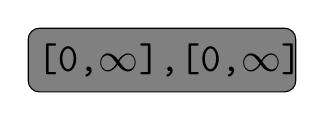
\begin{tikzpicture}
	\node [block3,fill = gray] (n2) {{\tt\Large [0,$\infty$],[0,$\infty$]}};
	\end{tikzpicture}
	}.
\end{center}
\item It enumerates 12 cases of refined features from $f = (\epsilon,([0,\infty],[0,\infty]),\epsilon)$ (e.g., 8 cases of \Append($f$) and 4 cases of \Replace($f$)).
It chooses the following feature produced from \Replace($f$):
\begin{center}
\resizebox{0.18\columnwidth}{!}{
	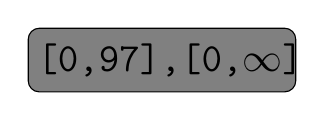
\begin{tikzpicture}
	\node [block3,fill = gray] (n2) {{\tt\Large [0,97],[0,$\infty$]}};
	\end{tikzpicture}}
\end{center}
 which has the highest score 0.06 among the 12 cases of features.
\item Because the score is less than $0.5$,
it refines the feature again to the following specific one, which comes from $\Append(\epsilon,([0,97],[0,\infty]),\epsilon),$ with the same manner:
\begin{center}
\resizebox{0.4\columnwidth}{!}{
	\begin{tikzpicture}
	\node [block3,fill = gray] (n2) {{\tt\Large [0,97],[0,$\infty$]}};
	\node [block3,right = 0.8cm of n2] (n3) {{\tt\Large [97,$\infty$],[0,$\infty$]}};
	\path [line] (n2) -> (n3);
	\end{tikzpicture}
	}
\end{center}
where the feature has score 0.23.
\item To find a better one, it refines the feature further; it enumerates 16 cases of refined features (e.g., 8 cases for replacing and 8 cases for appending a node). The following feature is selected:
\begin{center}
\resizebox{0.4\columnwidth}{!}{
	\begin{tikzpicture}
	\node [block3,fill = gray] (n2) {{\tt\Large [0,97],[0,$\infty$]}};
	\node [block4,right = 0.8cm of n2] (n3) {{\tt\Large [97,$\infty$],[140,$\infty$]}};
	\path [line] (n2) -> (n3);
	\end{tikzpicture}
	}
\end{center}
where the score is 0.37.
\item In the next iteration, it finally finds an informative feature which has a score 0.55:
\begin{center}
\resizebox{0.4\columnwidth}{!}{
	\begin{tikzpicture}
	\node [block3,fill = gray] (n2) {{\tt\Large [0,48],[0,$\infty$]}};
	\node [block4,right = 0.8cm of n2] (n3) {{\tt\Large [97,$\infty$],[140,$\infty$]}};
	\path [line] (n2) -> (n3);
	\end{tikzpicture}
	}.
\end{center}
\end{enumerate}





















% !TEX root = ./paper.tex

\section{Evaluation}
In this section, we experimentally evaluate our technique for learning graph-based heuristics.
We aim to answer the following research questions:

\begin{itemize}
\item {\bf Effectiveness and Generality:}
How effectively does the learned heuristic perform compared to the state-of-the-art heuristics?
Is it generally applicable for different analysis tasks without manual effort for designing application-specific features?

\item {\bf Learning Algorithm:}
How much does the learning cost?
How does the hyper-parameter $\hyper$ affect the performance of the learned heuristics?

% i.e.,
%~\Scaler~\cite{Li2018b},~\Zipper~\cite{Li2018a},~\Data~\cite{JeJeChOh17},~\Mahjong~\cite{Tan2017}?
\item {\bf Learned Insight:}
Does our approach produce explainable heuristics?
What are the insights learned from the generated heuristics?
\end{itemize}

\myparagraph{Overall Setting}
We implemented our approach, as a tool \OurCtx, on top of \Doop~\cite{BravenboerS09},
a pointer analysis framework for Java that has been widely used in prior works
~\cite{Smaragdakis2014,JeJeChOh17,JeJeOh18,Tan2017,TanLX16}.
%In particular, we applied our approach to learn heap abstraction and context-sensitivity heuristics from FPG and OAG, respectively.
%We implemented our technique on the two different artifacts~\cite{Tan2017,Li2018b}, the state-of-the-art context-sensitivity and heap abstraction heuristics, to demonstrate the effectiveness of our learned heuristics on both heuristics.
For the precision and scalability metrics, we follow existing works~\cite{Tan2017,Li2018a,Li2018b,JeJeChOh17} and use the number of may-fail casts alarms and the time spent on each analysis.
We also use the number of polymorphic call sites (i.e. call sites whose targets are not uniquely determined by each pointer analysis) and call-graph edges as additional precision metrics. For all precision metrics, the lower is the better.
%Polymorphic call sites present call sites that are not disambiguated into monomorphic calls.
We set the time budget as 3 hours (10,800 sec) for all analyses.
For the hyper-parameter $\hyper$, we chose the one among various values (e.g., 0.1, 0.2, ..., 0.9) via cross validation (we explain how this is done in section~\ref{sec:learning_alg}).
For each feature, we limit it to have at most three nodes due to scalability.
All the experiments were done on a machine with i7 CPU and 64 GB RAM running Ubuntu 16.04 (64bit).
We used the OpenJDK (1.6.0\_24) library.


%\myparagraph{Benchmarks}
We used a total of 17 programs: 10 programs (luindex, lusearch, antlr, pmd$_{m}$, chart, eclipse, fop, bloat, xalan, and jython) from the DaCapo 2006-10-MR2 benchmark suite~\cite{Blackburn2006}
and 7 programs (pmd$_{s}$, jedit, briss, soot, findbugs, JPC, and checkstyle) obtained from the artifacts provided by~\cite{Tan2017} and~\cite{Li2018b}.
%Here, we used two different versions of pmd where pmd$_{m}$ is a program in Dacapo benchmarks used in~\cite{Tan2017}, and pmd$_{s}$ is an open-source application used in~\cite{Li2018b}.
Here, we used two different versions of pmd where pmd$_{m}$ is a small program used by~\cite{Tan2017}, and pmd$_{s}$ is an open-source application used by~\cite{Li2018b}.
We split the benchmark programs into training, validation, and test sets.
The training and validation sets are used for learning a heuristic, and the test set is used for evaluating the performance of the learned heuristic.
For the training set, we used relatively small benchmarks, because our algorithm includes a process
to obtain minimal abstractions and this task is too expensive to run for large programs.
The validation set is used for choosing the hyper-parameter $\hyper$; we chose the one that leads the heuristic to the best performance on the validation set.
%After training heuristics with various values of $\hyper$, we chose the one which shows the best performance on a validation program {\tt findbugs}.
%We discuss the importance of the value of $\hyper$ later in detail.


\subsection{Effectiveness and Generality}
We demonstrate the effectiveness and generality of our technique by comparing it with two state-of-the-art graph-based heuristics: \Scaler~\cite{Li2018b} and \Mahjong~\cite{Tan2017}.

%comparing the performance of the generated heuristics to existing context-sensitivity heuristics and heap abstraction heuristics.

\subsubsection{Comparison with Scaler}\label{sec:comparescaler}
%\textcolor{black}{
\myparagraph{Setting}
\Scaler~is a context-sensitivity heuristic that works on the object allocation graph (OAG)~\cite{Li2018b}. From the OAG, it infers a policy to assign one of 2-object-sensitivity, 2-type-sensitivity, 1-type-sensitivity, and context-insensitivity to each method.
We used the same pre-analysis of \Scaler~to obtain the OAG and let our technique produce a heuristic.
We set $\CallDepth$ in Section~\ref{sec:param-context} to 3, where 0, 1, 2, and 3 correspond to context-insensitivity, 1-type-sensitivity, 2-type-sensitivity, and 2-object-sensitivity, respectively.
Unlike \Scaler, our heuristic assigns a context for each heap allocation site.
It poses $4^N$ possibilities where $N$ denotes the number of allocation-sites in the program.
%}
%as Scaler does.}
% that assigns one of the four context-sensitivity options to each method call.
%To compare with existing context-sensitivity heuristics, we learned such heuristics using the object-allocation-graphs (OAG) on which the state-of-the-art context-sensitivity heuristic \Scaler~was developed.
%For fair comparison, our learned heuristic,~\OurCtx, assigns either 2-object-sensitivity, 2-type-sensitivity, 1-type-sensitivity, or context-insensitive analysis to each method call as \Scaler~does.
%We also apply 2-object-sensitivity if receiver objects have a type \emph{java.util.*}, like \Scaler~does to preserve the precision.
%In our framework, since we explained that object-sensitivity heuristics assign different depth (e.g., 0,1, or 2) of context to each method call, these four analysis heuristics correspond to 3, 2, 1, and 0, respectively.
%This abstraction still satisfies the monotonicity as 2-object-sensitivity is strictly more precise than 2-type-sensitivity~\cite{Smaragdakis2011}.

Although the primary  objective in this evaluation is to compare with \Scaler, we evaluated two more heuristics as well: \Zipper~\cite{Li2018a} and \Data~\cite{JeJeChOh17}.
\Zipper~is another graph-based context-sensitivity heuristic that works on the precision flow graph (PFG).
\Data~is not graph-based, but we include it because \Data~is currently the state-of-the-art data-driven pointer analysis algorithm (with hand-crafted features).
%n object-sensitivity heuristic from machine learning technique with hand crafted features~\cite{JeJeChOh17}.
%the three graph-based heuristics \OurCtx,\Scaler, and \Zipper~use context-insensitive analysis as a pre-analysis to obtain a graph.
%Meanwhile, \Data~is another object-sensitivity heuristic from machine learning technique with hand crafted features~\cite{JeJeChOh17}.
In short, we compare the following pointer analysis algorithms: %to demonstrate the effectiveness of our learned context-sensitivity heuristic:

\begin{itemize}
\item \Scaler: A hand-crafted graph-based object-sensitivity heuristic for OAG~\cite{Li2018b}
\item \OurCtx: Our learning-based graph-based object-sensitivity heuristic for OAG
\item \Zipper: A hand-crafted graph-based object-sensitivity heuristic for PFG~\cite{Li2018a}
\item \Data: A state-of-the-art learning-based object-sensitivity heuristic~\cite{JeJeChOh17}
\item \twoobjH: The 2-object-sensitivity with 1-context-sensitive heap (precision upper bound)
\item \Insens: The context-insensitive analysis (scalability upper bound)
\end{itemize}
%  All heuristics use allocation-site-based heap abstraction.
%Our framework generated 195 features in total as an object-sensitivity heuristic (e.g., 68 features for 2-object-sensitivity, 28 for 2-type-sensitivity, and 99 features for 1-type-sensitivity).
%The learning procedure takes about 220 hours in total, where 168 hours are for getting minimal abstractions over the training programs
%and 52 hours for generating the features.


%To compare~\OurCtx~with~\Scaler,
We used three programs (luindex, lusearch, antlr) as the training set, one program (findbugs) as the validation set,
and the remaining thirteen programs (pmd$_{s}$, chart, eclipse, jedit, briss, soot, jython, pmd$_{m}$, fop, bloat, JPC, checkstyle, xalan) as the test set.
We chose findbugs as a validation program because it is a popular Java application and
requires suitable heuristics to be analyzed cost-effectively.
For example, \twoobjH~does not terminate on this program even after thousands of seconds or more.


\myparagraph{Results}
\begin{table}[]
\setlength\extrarowheight{-1pt}
\caption{Performance of the context-sensitivity heuristics against benchmarks.
%For all metrics, the lower is the better.
%For precision metric, we use the number of may-fail casts(\#may-fail casts) and polymorphic call sites (\#poly-call sites) whose targets are not uniquely determined by each pointer analysis.
%For scalability metric, we use analysis time, and the number in a parenthesis presents the sum of time spent during pre-analysis process.
%\#call-graph-edges for the training and validation programs are omitted due
%    to the lack of space.
}
\label{tbl:contextAbstraction}
\scriptsize
\begin{tabular}{@{}r|clrrrrrr@{}}
\toprule
\multicolumn{1}{c}{}               &                           & \multicolumn{1}{c}{} & \multicolumn{1}{c}{\OurCtx} & \multicolumn{1}{c}{\Scaler} & \multicolumn{1}{c}{\Zipper} & \multicolumn{1}{c}{\Data} & \multicolumn{1}{c}{\twoobjH} & \multicolumn{1}{c}{\Insens} \\ \midrule
\multirow{9}{*}{\rotatebox[origin=c]{90}{Training programs}} & \multirow{3}{*}{luindex}  & analysis time (s)    & 22(+22)                       & 36(+17)                         & 33(+17)                         & 19                         & 36                       & 15                         \\
                                   &                           & \#may-fail casts     & 297                      & 297                        & 310                        & 341                         & 297                      & 734                        \\
                                   &                           & \#poly-call sites    & 682                      & 675                        & 677                        & 702                         & 675                         & 940                        \\
                                   %&                           & \#call-graph-edges   & 29,045                   & 29,021                     & 29,025                     & 29,196                         & 29,021                         & 33,130                      \\
\cmidrule(){2-9}
                                   & \multirow{3}{*}{lusearch} & analysis time (s)    & 24(+21)                       & 63(+15)                         & 62(+17)                         & 19                         & 66                       & 15                         \\
                                   &                           & \#may-fail casts     & 299                      & 299                        & 305                        &  347                        & 299                      & 844                        \\
                                   &                           & \#poly-call sites    & 858                      & 850                        & 853                        & 883                         & 850                         & 1,133                      \\
                                   %&                           & \#call-graph-edges   & 31,838                   & 31,811                     & 31,817                     & 31,995                         & 31,811                         & 36,343                      \\
\cmidrule(){2-9}
                                   & \multirow{3}{*}{antlr}    & analysis time (s)    & 50(+94)                       & 51(+24)                         & 84(+26)                           & 33                         & 109                      & 24                         \\
                                   &                           & \#may-fail casts     & 409                      & 412                        & 420                           & 513                         & 409                      & 918                        \\
                                   &                          & \#poly-call sites    & 1,495                    & 1,488                      & 1,488                           & 1,517                         & 1,487                         & 1,729                      \\
                                   %&                           & \#call-graph-edges   & 47,273                   & 49,398                     & 47,233                           & 47,358                         & 47,232                         & 50,652                      \\
\midrule \midrule
\multirow{28}{*}{\rotatebox[origin=c]{90}{Test programs}} & \multirow{4}{*}{pmd$_{s}$}      & analysis time (s)    & 710(+92)                      & 494(+49)                        &  $>$10,800                          & 117                         & $>$10,800     & 48                         \\
                                   &                           & \#may-fail casts     & 2,075                    & 2,176                      & -                           & 2,145                         & -                         & 2,948                      \\
                                   &                           & \#poly-call sites    & 3,507                    & 3,536                      & -                           & 3,647                         & -                         & 4,183                      \\
                                   &                           & \#call-graph-edges   & 92,589                   & 92,775                     & -                           & 94,328                         & -                         & 104,457                     \\\cmidrule(){2-9}

                                   & \multirow{4}{*}{chart}    & analysis time (s)    & 63(+73)                       & 184(+48)                        & 113(+56)                        & 35                         & 196                      & 48                       \\
                                   &                           & \#may-fail casts     & 998                      & 976                        & 888                        & 974                         & 883                      & 1,810                         \\
                                   &                           & \#poly-call sites    & 1,392                    & 1,402                      & 1,379                      & 1,435                         & 1,378                         & 1,852                      \\
                                   &                           & \#call-graph-edges   & 52,544                   & 53,198                     & 52,377                     & 52,647                         & 52,374                         & 63,453                     \\\cmidrule(){2-9}
                                   & \multirow{4}{*}{eclipse}  & analysis time (s)    & 1,395(+103)                    & 652(+92)                        & 9,701(+114)                           & 159                         & $>$10,800     & 91                         \\
                                   &                           & \#may-fail casts     & 2,989                    & 3,211                      & 2,897                           & 3,178                         & -                         & 4,190                      \\
                                   &                           & \#poly-call sites    & 8,418                    & 8,486                      & 8,390                           & 8,627                         & -                         & 9,197                      \\
                                   &                           & \#call-graph-edges   & 144,873                  & 145,953                    & 143,727                           & 146,512                         & -                         & 161,222                     \\\cmidrule(){2-9}
                                   & \multirow{4}{*}{jedit}    & analysis time (s)    & 845(+90)                      & 1,377(+79)                      &   $>$10,800                         & 137                         & $>$10,800      & 78                         \\
                                   &                           & \#may-fail casts     & 2,196                    & 2,397                      &  -                          & 2,298                         &  -                        & 3,398                      \\
                                   &                           & \#poly-call sites    & 3,917                    & 4,012                      &  -                          & 4,091                         &  -                        & 4,769                      \\
                                   &                           & \#call-graph-edges   & 98,401                   & 99,536                     &  -                          & 99,697                         &  -                        & 120,309                     \\\cmidrule(){2-9}
                                   & \multirow{4}{*}{briss}    & analysis time (s)    & 2,368(+169)                    & 907(+151)                           & $>$10,800                           & 499                         & $>$10,800     & 149                        \\
                                   &                           & \#may-fail casts     & 3,065                    & 3,428                      &  -                          & 3,162                         &  -                        & 4,904                      \\
                                   &                           & \#poly-call sites    & 5,099                    & 5,323                      &  -                          & 5,291                         &  -                        & 6,297                      \\
                                   &                           & \#call-graph-edges   & 150,351                  & 152,761                    &  -                          & 151,861                         &  -                        & 176,785                     \\\cmidrule(){2-9}
                                   & \multirow{4}{*}{soot}     & analysis time (s)    & $>$10,800     & 883(+727)                        & $>$10,800                           & $>$10,800                         & $>$10,800     & 698                        \\
                                   &                           & \#may-fail casts     &  -                        & 10,549                     &   -                         & -                         &   -                       & 16,570                     \\
                                   &                           & \#poly-call sites    &  -                        & 14,822                     &   -                         & -                         &   -                       & 16,532                     \\
                                   &                           & \#call-graph-edges   &  -                        & 374,877                    &  -                          & -                         &  -                        & 415,476                     \\\cmidrule(){2-9}
                                   & \multirow{4}{*}{jython}   & analysis time (s)    & $>$10,800     & 314(+96)                        & $>$10,800                           & 425                         & $>$10,800     & 73                         \\
                                   &                           & \#may-fail casts     & -                         & 1,852                      &  -                          & 1,773                          &  -                        & 2,234                      \\
                                   &                           & \#poly-call sites    & -                         & 2,500                      &  -                          & 2,481                         & -                         & 2,778                      \\
                                   &                           & \#call-graph-edges   &  -                        & 107,410                     & -                           & 106,837                         &  -                        & 114,856
\\\midrule \midrule
\multirow{3}{*}{\rotatebox[origin=c]{90}{Valid}}
                                   & \multirow{3}{*}{findbugs} & analysis time (s)    & 305(+58)                      & 191(+36)                        & 1,399(+43)                           & 59                         & 2,458                    & 35                      \\
                                   &                           & \#may-fail casts     & 1,436                    & 1,452                      & 1,412                           & 1,663                         & 1,409                    & 2,508                         \\
                                   &                           & \#poly-call sites    & 2,188                    & 2,195                      & 2,182                           & 2,220                         & 2,182                         & 2,925                      \\
                                   %&                           & \#call-graph-edges   & 65,874                   & 66,177                     &  65,838                          & 66,028                         &  65,836                        & 77,370                     \\
\bottomrule
\end{tabular}
\end{table} 

% Please add the following required packages to your document preamble:
% \usepackage{booktabs}
% \usepackage{multirow}
\begin{table}[]
\setlength\extrarowheight{-1pt}
\caption{Performance comparison among various context sensitivity heuristics against the left six benchmarks. All the notations are the same with Table~\ref{tbl:contextAbstraction}.}
\label{appendix:ctx}
\centering
\footnotesize
\begin{tabular}{@{}c|clrrrrrr@{}}
\toprule
\multicolumn{1}{c}{}&\multicolumn{1}{c}{}        & \multicolumn{1}{c}{} & \multicolumn{1}{c}{\OurCtx} & \multicolumn{1}{c}{\Scaler} & \multicolumn{1}{c}{\Zipper} & \multicolumn{1}{c}{\Data} & \multicolumn{1}{c}{\twoobjH} & \multicolumn{1}{c}{\Insens} \\ \midrule
\multirow{28}{*}{\rotatebox[origin=c]{90}{Test programs}}&\multirow{4}{*}{pmd$_m$}       & analysis time (s)    & 43(+67)                      & 55(+44)                    & 57(+78)                    & 30                       & 67                       & 23                         \\
&                            & \#may-fail casts     & 288                          & 287                        & 300                        & 327                      & 287                      & 679                        \\
&                            & \#poly-call sites    & 643                          & 636                        & 638                        & 667                      & 636                      & 885                        \\%\cmidrule(){2-9}
&                            & \#call-graph-edges   & 27,074                        & 27,052                      & 27,056                      & 27,147                    & 27,052                    & 30,328                      \\\cmidrule(){2-9}
&\multirow{4}{*}{fop}        & analysis time (s)    & 212(+88)                     & 341(+54)                   & 533(+71)                   & 74                       & 949                      & 53                         \\
&                            & \#may-fail casts     & 1,568                         & 1,732                       & 1,449                       & 1,600                     & 1,446                     & 2,458                       \\
&                            & \#poly-call sites    & 2,876                         & 2,945                       & 2,848                       & 3,009                     & 2,844                     & 3,585                       \\%\cmidrule(){2-9}
&                            & \#call-graph-edges   & 71,612                        & 72,556                      & 71,418                      & 72,113                    & 71,408                    & 84,330                      \\\cmidrule(){2-9}
&\multirow{4}{*}{bloat}      & analysis time (s)    & 216(+30)                     & 290(+21)                   & 2402(+23)                  & 44                       & 2,422                     & 20                         \\
&                            & \#may-fail casts     & 1,215                         & 1,222                       & 1,205                       & 1,288                     & 1,193                     & 1,924                       \\
&                            & \#poly-call sites    & 1,458                         & 1,465                       & 1,429                       & 1,496                     & 1,427                     & 2,014                       \\%\cmidrule(){2-9}
&                            & \#call-graph-edges   & 53,641                        & 53,867                      & 53,147                      & 54,059                    & 53,143                    & 61,150                      \\\cmidrule(){2-9}
&\multirow{4}{*}{JPC}        & analysis time (s)    & 118(+69)                     & 274(+38)                   & 266(+55)                   & 45                       & 398                      & 37                         \\
&                            & \#may-fail casts     & 1,427                         & 1,552                       & 1,343                       & 1,472                     & 1,345                     & 2,261                       \\
&                            & \#poly-call sites    & 4,210                         & 4,228                       & 4,187                       & 4,322                     & 4,186                     & 4,924                       \\%\cmidrule(){2-9}
&                            & \#call-graph-edges   & 79,912                        & 80,098                      & 79,787                      & 80,208                    & 79,783                    & 94,569                      \\\cmidrule(){2-9}
&\multirow{4}{*}{checkstyle} & analysis time (s)    & 133(+70)                     & 264(+45)                   & 396(+52)                   & 69                       & 1,693                     & 44                         \\
&                            & \#may-fail casts     & 600                          & 625                        & 590                        & 644                      & 581                      & 1,114                       \\
&                            & \#poly-call sites    & 1,052                         & 1,038                       & 1,040                       & 1,089                     & 1,035                     & 1,444                       \\%\cmidrule(){2-9}
&                            & \#call-graph-edges   & 9,516                         & 9,514                       & 48,830                      & 48,996                    & 48,809                    & 57,490                      \\\cmidrule(){2-9}
&\multirow{4}{*}{xalan}      & analysis time (s)    & 226(+64)                     & 539(+38)                   & 119(+45)                   & 44                       & 881                      & 37                         \\
&                            & \#may-fail casts     & 567                          & 579                        & 556                        & 604                      & 533                      & 1,182                       \\
&                            & \#poly-call sites    & 1,533                         & 1,523                       & 1,533                       & 1,583                     & 1,522                     & 1,898                       \\%\bottomrule
&                            & \#call-graph-edges   & 45,269                        & 44,887                      & 9,125                       & 45,549                    & 44,871                    & 5,1302                      \\ \bottomrule 
\end{tabular}
\end{table}


%\myparagraph{Result of context-sensitivity heuristic}
Table~\ref{tbl:contextAbstraction} and~\ref{appendix:ctx} present the performance of the context-sensitivity heuristics described above.
The number in a parenthesis for graph-based heuristics (i.e. \OurCtx, \Zipper, and \Scaler)
represents the sum of time spent on performing the pre-analysis (i.e. context-insensitive analysis) and running the heuristics on the graphs for extracting context abstractions.

The results show that our technique can automatically generate a cost-effective heuristic that performs as competitive as the state-of-the-art object-sensitivity heuristics.
%In comparison to the baseline heuristic~\Scaler, which employs the same graph OAG, \OurCtx~consistently shows a better precision than \Scaler~
%with some losses in scalability.
Compared to the baseline heuristic~\Scaler, which employs the same graph OAG, \OurCtx~%consistently
shows a better precision than \Scaler~
with some losses in scalability for the test programs pmd$_{s}$, eclipse, and briss.
For example, \OurCtx~reports 101 less may-fail casts alarms than \Scaler~ for the test program pmd$_{s}$
while taking 216 more seconds.
In addition, \OurCtx~shows better performance in both precision and scalability than \Scaler~on the test programs (except pmd$_m$) in Table~\ref{appendix:ctx}.
For example, in jedit, \OurCtx~produces 201 less alarms with 35\% less analysis time.
In comparison to \Zipper, \OurCtx~consistently outperforms in scalability.
For example, \OurCtx~successfully analyzed pmd$_{s}$, jedit, and briss with remarkably less costs when \Zipper~fails to analyze them within the time budget.
In comparison to \Data, the result shows that \OurCtx~performs far better in precision.
%Although \Data~presents better scalability than \OurCtx, it produces about 100$\sim$300 \TODO{concrete numbers} more alarms for the testing programs.
Although \Data~presents better scalability than \OurCtx, it produces more than 92 alarms for the test programs pmd$_{s}$, eclipse, jedit and briss.
Compared to \twoobjH, \OurCtx~ shows better performance in scalability for the majority of test programs which \twoobjH~fails to analyze within the given time budget (3 hours).

\subsubsection{Comparison with Mahjong}\label{sec:eval_heap}
\myparagraph{Setting}
%To show the generality of our framework,
%we additionally evaluated our technique to learn a graph-based heap abstraction heuristic from field points-to graph (FPG) which the state-of-the-art heap abstraction heuristic \Mahjong~uses.

\Mahjong~is a graph-based heap abstraction heuristic that works on the field points-to graph (FPG)~\cite{Tan2017}.
From the FPG, which is obtained by running a context-insensitive pre-analysis, \Mahjong~infers a policy that determines whether to merge objects allocated in different allocation sites.
We used the same pre-analysis to obtain the FPG and let our technique produce a heap abstraction heuristic.
Unlike \Mahjong, our heap abstraction heuristic (i.e. \OurHeap) assigns `{\it type}' (type-based heap abstraction) or `{\it alloc}' (allocation-site-based heap abstraction) to each heap allocation-site which poses
$2^N$ possibilities where $N$ denotes the number of allocation-sites in the program.
%\todored{needs more explanation how $2^\mbh$ possibilities are selected...}
We compare the following four analyses:
\begin{itemize}
\item \Mahjong: The state-of-the-art graph-based heap abstraction heuristic~\cite{Tan2017}
\item \OurHeap: Our learning-based graph-based heap abstraction heuristic
\item \AllocBased: The uniform allocation-site-based heap abstraction (precision upper bound)
\item \TypeBased: The uniform type-based heap abstraction (scalability upper bound)
\end{itemize}
Following \Mahjong~\cite{Tan2017}, all analyses above use 3-object-sensitivity with 2-context-sensitive heap.

For this evaluation, we used the same benchmark programs in the section~\ref{sec:comparescaler}.
We used four programs (luindex, lusearch, antlr, pmd$_{m}$) as the training set and
twelve programs (fop, chart, bloat, xalan, JPC, checkstype, eclipse, pmd$_{s}$, jecit, briss, soot, jython) as the test set.
We also used findbugs as a validation program.
% as we did for the comparison with~\Scaler
%From the 17 benchmarks, we used four programs (luindex, lusearch, antlr, pmd$_{m}$) as the training set.


\begin{table}[]
\setlength\extrarowheight{-1.5pt}
\caption{Performance of the heap abstraction heuristics against benchmarks.
The notions are the same with those in Table~\ref{tbl:contextAbstraction}.}
\label{tbl:heapAbstraction}
\centering
\scriptsize
\begin{tabular}{@{}c|clrrrr@{}}
\toprule
\multicolumn{1}{c}{}                                    &                             &                    & \multicolumn{1}{c}{\OurHeap} & \multicolumn{1}{c}{\Mahjong} & \multicolumn{1}{c}{\AllocBased} & \multicolumn{1}{c}{\TypeBased} \\ \midrule
\multirow{16}{*}{\rotatebox[origin=c]{90}{Training programs}} & \multirow{4}{*}{luindex}    & analysis time(s)   & 23(+90)                       & 42(+21)                          & 5,475                           & 19                             \\
                                   &                             & \#may-fail casts   & 358                      & 358                         & 358                             & 795                            \\
                                   &                             & \#poly-call sites  & 928                      & 918                         & 915                             & 1,128                          \\
                                   &                             & \#call-graph-edges & 33,450                   & 33,365                      & 33,356                          & 37,898                         \\ \cmidrule(l){2-7}
                                   & \multirow{4}{*}{lusearch}   & analysis time(s)   & 21(+92)                       & 43(+19)                          & \textgreater{}10,800            & 19                             \\
                                   &                             & \#may-fail casts   & 372                      & 372                         & -                               & 884                            \\
                                   &                             & \#poly-call sites  & 1,127                    & 1,116                       & -                               & 1,331                          \\
                                   &                             & \#call-graph-edges & 36,298                   & 36,237                      & -                               & 41,211                         \\ \cmidrule(l){2-7}
                                   & \multirow{4}{*}{antlr}      & analysis time(s)   & 31(+101)                       & 48(+33)                          & 5,241                           & 26                             \\
                                   &                             & \#may-fail casts   & 463                      & 463                         & 463                             & 1,002                           \\
                                   &                             & \#poly-call sites  & 1,630                    & 1,626                       & 1,623                           & 1,836                          \\
                                   &                             & \#call-graph-edges & 51,058                   & 51,043                      & 51,035                          & 55,745                         \\ \cmidrule(l){2-7}
                                   & \multirow{4}{*}{pmd$_{m}$}        & analysis time(s)   & 44(+137)                       & 88(+34)                          & 9,146                           & 42                             \\
                                   &                             & \#may-fail casts   & 871                      & 871                         & 871                             & 1,418                           \\
                                   &                             & \#poly-call sites  & 1,142                    & 1,133                       & 1,130                           & 1,388                          \\
                                   &                             & \#call graph edges & 44,094                   & 4,4016                      & 44,004                          & 50,365                         \\ \midrule \midrule
\multirow{24}{*}{\rotatebox[origin=c]{90}{Test programs}} & \multirow{4}{*}{fop}        & analysis time(s)   & 30(+117)                       & 50(+26)                          & 5,475                            & 33                            \\
                                   &                             & \#may-fail casts   & 376                      & 375                         & 375                             & 779                             \\
                                   &                             & \#poly-call sites  & 830                      & 817                         & 814                             & 1,034                          \\
                                   &                             & \#call graph edges & 34,259                   & 34,192                      & 34,184                          & 38,629                         \\ \cmidrule(l){2-7}
                                   & \multirow{4}{*}{chart}      & analysis time(s)   & 436(+350)                      & \textgreater 10,800         & \textgreater 10,800             & 199                             \\
                                   &                             & \#may-fail casts   & 1,331                     & -                           & -                               & 2,299                           \\
                                   &                             & \#poly-call sites  & 2,078                    & -                           & -                               & 2,363                          \\
                                   &                             & \#call graph edges & 72,746                   & -                           & -                               & 82,952                         \\ \cmidrule(l){2-7}
                                   & \multirow{4}{*}{bloat}      & analysis time(s)   & 376(+121)                      & \textgreater 10,800         & \textgreater 10,800             & 26                             \\
                                   &                             & \#may-fail casts   & 1,247                     & -                           & -                               & 1,926                           \\
                                   &                             & \#poly-call sites  & 1,593                    & -                           & -                               & 1,793                          \\
                                   &                             & \#call graph edges & 56,535                   & -                           & -                               & 64,220                         \\ \cmidrule(l){2-7}
                                   & \multirow{4}{*}{xalan}      & analysis time(s)   & 489(+162)                      & 795(+29)                         & \textgreater 10,800             & 59                             \\
                                   &                             & \#may-fail casts   & 539                      & 535                         & -                               & 1,093                           \\
                                   &                             & \#poly-call sites  & 1,601                    & 1,591                       & -                               & 1,876                          \\
                                   &                             & \#call graph edges & 46,026                   & 45,950                      & -                               & 51,761                         \\ \cmidrule(l){2-7}
                                   & \multirow{4}{*}{JPC}        & analysis time(s)   & 1,730(+366)                    & 3,309(+47)                       & \textgreater 10,800             & 524                            \\
                                   &                             & \#may-fail casts   & 1,300                    & 1,226                       & -                               & 2,007                          \\
                                   &                             & \#poly-call sites  & 4,211                    & 4,139                       & -                               & 4,646                          \\
                                   &                             & \#call graph edges & 79,864                   & 79,370                      & -                               & 91,248                         \\ \cmidrule(l){2-7}
                                 & \multirow{4}{*}{checkstyle} & analysis time(s)   & 1,333(+563)                    & 2,346(+53)                       & \textgreater 10,800             & 48                             \\
                                   &                             & \#may-fail casts   & 1,085                    & 1,022                       & -                               & 1,749                          \\
                                   &                             & \#poly-call sites  & 2,202                    & 2,168                       & -                               & 2,489                          \\
                                   &                             & \#call-graph-edges & 66,321                   & 65,943                      & -                               & 77,962                         \\
\midrule\midrule
\multirow{3}{*}{\rotatebox[origin=c]{90}{Valid}}
& \multirow{3}{*}{findbugs}   & analysis time(s)   & 96(+363)                       & 273(+70)                         & \textgreater 10,800             & 92                             \\
                                   &                             & \#may-fail casts   & 1,774                    & 1,671                       & -                               & 3,089                          \\
                                   &                             & \#poly call sites  & 3,576                    & 3,534                       & -                               & 4,281                          \\
%                                   &                             & \#call graph edges & 87,459                   & 86,985                      & -                               & 16,876                         \\
 \bottomrule
\end{tabular}
\end{table}


% Please add the following required packages to your document preamble:
% \usepackage{booktabs}
% \usepackage{multirow}
\begin{table}[]
\scriptsize
\centering
\caption{Performance comparison between the heap abstraction heuristics against the left benchmarks.}
\label{appendix:heap}
\begin{tabular}{@{}c|clrrrr@{}}
\toprule
\multicolumn{1}{c}{}&                         &                    & \OurHeap             & \Mahjong              & \AllocBased         & \TypeBased          \\ \midrule
\multirow{28}{*}{\rotatebox[origin=c]{90}{Test programs}}&\multirow{4}{*}{eclipse} & analysis time (s)  & $>$10,800 & $>$10,800 & $>$10,800 & 222                  \\
&                         & \#may-fail casts   & -                    & -                    & -                    & 4,852                 \\
&                         & \#poly-call sites  & -                    & -                    & -                    & 10,177                \\%\cmidrule(){2-7}
&                         & \#call-graph-edges & -                    & -                    & -                    & 182,000               \\\cmidrule(){2-7}
&\multirow{4}{*}{pmd$_s$}  & analysis time (s)  & $>$10,800 & $>$10,800 & $>$10,800 & 4,317                 \\
&                         & \#may-fail casts   & -                    & -                    & -                    & 2,941                 \\
&                         & \#poly-call sites  & -                    & -                    & -                    & 4,124                 \\%\cmidrule(){2-7}
&                         & \#call-graph-edges & -                    & -                    & -                    & 106,490               \\\cmidrule(){2-7}
&\multirow{4}{*}{jedit}   & analysis time (s)  & 454(+242)                  & 1,392                 & 8,001                 & 245                  \\
&                         & \#may-fail casts   & 1,143                 & 1,094                 & 1,094                 & 1,786                 \\
&                         & \#poly-call sites  & 1,732                 & 1,688                 & 1,684                 & 2,064                 \\%\cmidrule(){2-7}
&                         & \#call-graph-edges & 55,476                & 55,156                & 55,145                & 64,825                \\\cmidrule(){2-7}
&\multirow{4}{*}{briss}   & analysis time (s)  & $>$10,800 & $>$10,800 & $>$10,800 & $>$10,800 \\
&                         & \#may-fail casts   & -                    & -                    & -                    & -                    \\
&                         & \#poly-call sites  & -                    & -                    & -                    & -                    \\%\cmidrule(){2-7}
&                         & \#call-graph-edges & -                    & -                    & -                    & -                    \\\cmidrule(){2-7}
&\multirow{4}{*}{soot}    & analysis time (s)  & $>$10,800 & $>$10,800 & $>$10,800 & 7,741                 \\
&                         & \#may-fail casts   & -                    & -                    & -                    & 15,885                \\
&                         & \#poly-call sites  & -                    & -                    & -                    & 14,617                \\%\cmidrule(){2-7}
&                         & \#call-graph-edges & -                    & -                    & -                    & 359,358               \\\cmidrule(){2-7}
&\multirow{4}{*}{jython}  & analysis time (s)  & $>$10,800 & $>$10,800 & $>$10,800 & 187                  \\
&                         & \#may-fail casts   & -                    & -                    & -                    & 1,211                 \\
&                         & \#poly-call sites  & -                    & -                    & -                    & 1,487                 \\%\cmidrule(){2-7}
&                         & \#call-graph-edges & -                    & -                    & -                    & 50,544                \\ \bottomrule
\end{tabular}
\end{table}



\myparagraph{Results}
%\myparagraph{Result of the heap-abstraction heuristic}
Table~\ref{tbl:heapAbstraction} and~\ref{appendix:heap} show that our technique can produce a competitive graph-based heap abstraction heuristic from the FPG.
In comparison with \Mahjong, \OurCtx~shows a far better scalability while losing precision a bit.
\Mahjong~produced the same number of may-fail-casts with the most precise one, \AllocBased,
but it was unable to analyze large programs like {chart} and {bloat} within the time budget (3 hours).
Although \OurCtx~produced more alarms (103 at most) than \Mahjong, it successfully analyzed programs (i.e. chart and bloat) which \Mahjong~failed to analyze.
% within the given time budget.}
Currently, the overhead, the time taken by extracting an abstraction from the FPG, of our heuristic is bigger than \Mahjong~because \Mahjong~designed an efficient algorithm to produce an abstraction from FPG while ours is not optimized to minimize it. %, which is our future work to reduce the overhead.
The results, however, still demonstrate that \OurCtx~is competitive and has a strength in scalability compared to the state-of-the-art technique as it successfully analyzed the large programs, {chart} and {bloat}, which \Mahjong~ cannot handle.



\subsection{Learning Algorithm}\label{sec:learning_alg}

\myparagraph{Learning Cost }

To learn a context-sensitivity heuristic, our learning algorithm took 169 hours in total, where 144 hours are for getting minimal abstractions over the training programs and 25 hours for generating features.
To learn a heap abstraction heuristic, the algorithm took 107 hours, where 72 hours are for minimal abstraction generation and 35 hours for feature generation.
We note that, although the learning algorithm is expensive, it saves more expensive human costs by automating the manual process of designing analysis heuristics that would take weeks or months.


\begin{figure}
	\centering
	\begin{multicols}{2}
	\begin{subfigure}[t]{1.\columnwidth}
	\centering
	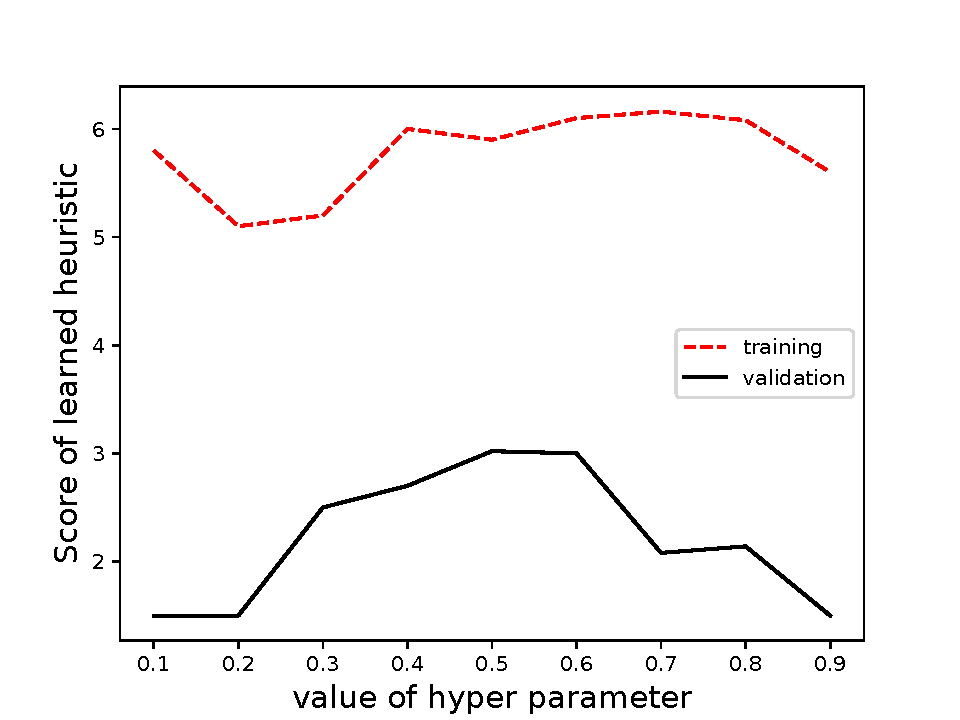
\includegraphics[width=6.3cm]{Graphick/figures/ctx_gamma.pdf}
	\caption{Object-sensitivity heuristic}
	\end{subfigure}
~\columnbreak

	\begin{subfigure}[t]{1.\columnwidth}
	\centering	
	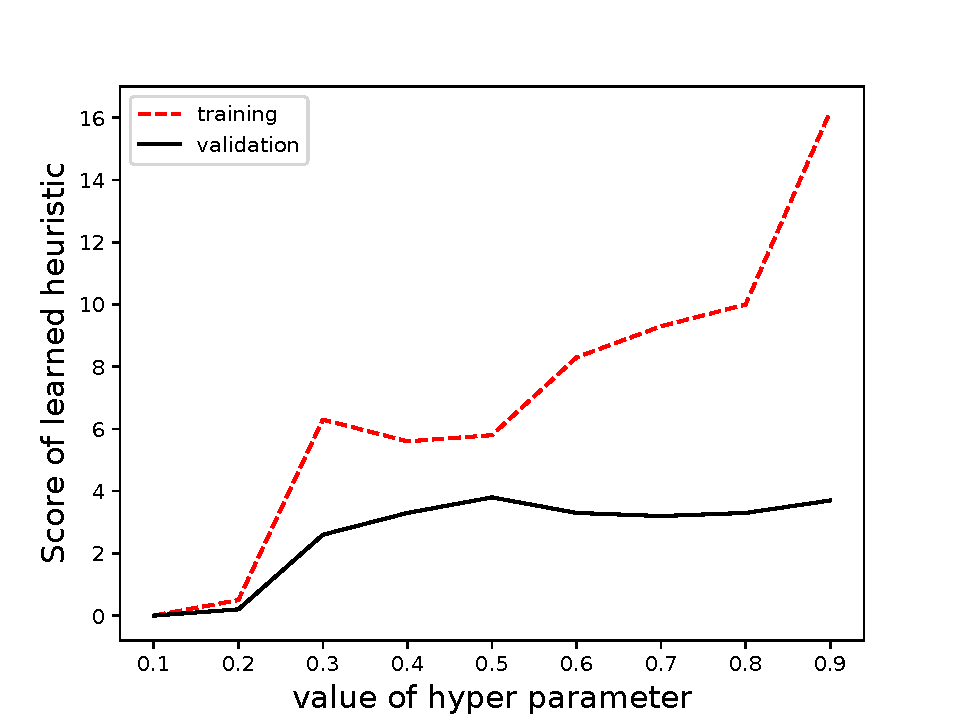
\includegraphics[width=6.3cm]{Graphick/figures/heap_gamma.pdf}
	\caption{Heap abstraction heuristic}
	\end{subfigure}
	\end{multicols}
	\caption{How score of learned heuristic changes over the value of $\hyper$.}
	\label{fig:gamma}
\end{figure}


\myparagraph{Choosing Hyper-Parameter $\hyper$}\label{sec:hyper_param}

Through our evaluation, we observed that the value of the hyper-parameter $\hyper$ plays an important role in the performance of the learned heuristic.
Figure~\ref{fig:gamma} depicts how performance of learned heuristics changes over the values of  $\hyper$.
The X-axis presents the value of $\hyper$ set to learn each heuristic, and
the Y-axis presents scores that we measured for performance of each heuristic $\heuristic_{\hyper}$ according to
${\sum_{P\in\vec{P}}\projproved(F_P(\heuristic_{\hyper}(G)))}\over{\sum_{P\in\vec{P}}
  \projcost(F_P(\heuristic_{\hyper}(G)))}$ where $\projcost$ denotes analysis time.
This score function presents the number of queries proved per second; thereby, more precise and scalable the analysis,
higher the score.
The red dotted and black solid lines present how the scores change over
the training programs $\vec{P}$ %(e.g., $\vec{P}$ = \{{\tt luindex,lusearch,antlr}\})
and the validation program, respectively.
For the training programs, the score of the learned heuristic increases as the higher $\hyper$ is given
because the heuristic becomes more fitted to the training programs.\footnote{It learned a bit bad heuristic when $\hyper$ is 0.9 in
  object-sensitivity heuristic because it is
difficult to generate specific features that satisfy such high precision
constraints; it eventually generates a general feature that include lots
of nodes.}
In our evaluation, both learned heuristics, however, perform the best on the validation program when $\hyper$ is 0.5;
thus, \OurCtx~in Table~\ref{tbl:contextAbstraction} and Table~\ref{tbl:heapAbstraction} corresponds to $\heuristic_{0.5}$.


%This occurs because the learned heuristics become overfitted to the training programs as the value of $\hyper$ increases;
%thus, simply increasing $\hyper$ is not an answer to achieve the best performance on validation and testing programs.







%\subsection{Learning Adequacy}

%\subsection{Insights from Generated Features}
\subsection{Learned Insights}

The learning algorithm generated 197 features in total for the object-sensitivity heuristic (68 features for 2-object-sensitivity, 29 for 2-type-sensitivity, and 100 features for 1-type-sensitivity). It generated 96 features for the heap abstraction heuristic.

\newcolumntype{P}[1]{>{\centering\arraybackslash}p{#1}}
\newcolumntype{M}[1]{>{\centering\arraybackslash}m{#1}}
\begin{figure}
\centering
\scriptsize
\setlength\extrarowheight{-1pt}
\begin{tabular}{|c|c|c| c | c | c |}
\toprule
\multicolumn{1}{|c}{}
                                                &                        & \multicolumn{1}{c|}{\textsf{Top 5 Features}} & \textsf{portion}
&\textsf{score} &
\multicolumn{1}{c|}{
\makecell{\textsf{Concretization}\\(Top 1)}
} \\ \midrule

\multirow{30}{*}{\rotatebox[origin=c]{90}{Object-Sensitivity Heuristic}}
& \multirow{10}{*}{\rotatebox[origin=c]{90}{1type}} &
\multirow{2}{*}{
\resizebox{0.40\columnwidth}{!}{
	\begin{tikzpicture}
	\node [block3,fill = gray] (n2) {{\tt\small [0,$\infty$],[61,$\infty$]}};
	\node [block3,right = 0.8cm of n2] (n3) {{\tt\small [46,$\infty$],[0,$\infty$]}};
	\path [line] (n2) -> (n3);
	\end{tikzpicture}
}
}
&\multirow{2}{*}{47\%} &\multirow{2}{*}{0.57}
                                        & \multirow{10}{*}{
		\resizebox{0.15\columnwidth}{!}{
			\begin{tikzpicture}
			\node [shape=circle,fill = gray,draw=black] (n1) {{\tt
                            n2}};
			\node [shape=circle,fill = gray,draw=black,left = 0.3cm
                        of n1] (n1left) {{\tt n1}};
			\node [shape=circle,fill = gray,draw=black,right = 0.3cm
                        of n1] (n1right) {{\tt n3}};
			\node [None,above = 0.7cm
                        of n1] (aboven1) {};
			\node [None,above = 0.7cm
                        of n1left] (aboven2) {};
			\node [None,above = 0.7cm
                        of n1right] (aboven3) {};
			\node [shape=circle,draw=black,below = 0.9cm
                        of n1] (n2) {{\tt n4}};
			\node [None,above left = 0.6 and 0.1cm
                        of n1] (n4) {};
			\node [None,right = 0.7cm
                        of n4] (n5) {};
			\node [None,above left = 0.7 and 0.5cm
                        of n2] (d1) {};
			\node [None, right = -0.1
                        of d1] (d2) {};
			\node [None, right = -0.1
                        of d2] (d3) {};
			\node [None, right = -0.1
                        of d3] (d4) {};
			\node [None, right = -0.1
                        of d4] (d5) {};
			\node [None, right = -0.1
                        of d5] (d6) {};
			\node [None, right = -0.1
                        of d6] (d7) {};
			\node [None, right = -0.1
                        of d7] (d8) {};
			\node [None, right = -0.1
                        of d8] (d9) {};
			\node [None, right = -0.1
                        of d9] (d10) {};
			\node [None, right = -0.1
                        of d10] (d11) {};
			\node [None, right = -0.1
                        of d11] (d12) {};
			\node [None, right = -0.1
                        of d12] (d13) {};		
			\path [line] (aboven1) -- (n1);
			\path [line] (aboven2) -- (n1left);
			\path [line] (aboven3) -- (n1right);
			\path [line] (n1left) -- (n2);
			\path [line] (n1right) -- (n2);
			\path [line] (n1) -- (n2);
			\path [line] (d1) -- (n2);
			\path [line] (d2) -- (n2);
			\path [line] (d3) -- (n2);
			\path [line] (d4) -- (n2);
			\path [line] (d5) -- (n2);
			\path [line] (d6) -- (n2);
			\path [line] (d7) -- (n2);
			\path [line] (d8) -- (n2);
			\path [line] (d9) -- (n2);
			\path [line] (d10) -- (n2);
			\path [line] (d11) -- (n2);
			\path [line] (d12) -- (n2);
			\path [line] (d13) -- (n2);
			\end{tikzpicture}
		}
}
                   \\
&&\multicolumn{1}{c|}{}&\multicolumn{1}{c|}{}  &\multicolumn{1}{c|}{}&\multicolumn{1}{c|}{}

\\
                                                &                        &
\multirow{2}{*}{
\resizebox{0.40\columnwidth}{!}{
	\begin{tikzpicture}
	\node [block3,fill = gray] (n2) {{\tt\small [0,$\infty$],[0,$\infty$]}};
	\node [block4,right = 0.8cm of n2] (n3) {{\tt\small [0,$\infty$],[117,$\infty$]}};
	\path [line] (n2) -> (n3);
	\end{tikzpicture}
}}
& \multirow{2}{*}{36\%} &\multirow{2}{*}{0.63}                                        &                                     \\
&&\multicolumn{1}{c|}{}&\multicolumn{1}{c|}{}  &\multicolumn{1}{c|}{}&\multicolumn{1}{c|}{}
\\
                                                &                        &
\multirow{2}{*}{
\resizebox{0.41\columnwidth}{!}{
	\begin{tikzpicture}
	\node [block4] (n2) {{\tt\small [0,$\infty$],[100,$\infty$]}};
	\node [block3,fill = gray,right = 0.8cm of n2] (n3) {{\tt\small [0,$\infty$],[29,$\infty$]}};
	\path [line] (n2) -> (n3);
	\end{tikzpicture}
}}
& \multirow{2}{*}{35\%} & \multirow{2}{*}{0.55}                                      &                                     \\
&&\multicolumn{1}{c|}{}&\multicolumn{1}{c|}{}  &\multicolumn{1}{c|}{}&\multicolumn{1}{c|}{}
\\
                                                &                        &
\multirow{2}{*}{
\resizebox{0.50\columnwidth}{!}{
	\begin{tikzpicture}
	\node [block4] (n2) {{\tt\small [0,$\infty$],[100,$\infty$]}};
	\node [block3,fill = gray,right = 0.3cm of n2] (n3) {{\tt\small [0,$\infty$],[0,$\infty$]}};
	\node [block4,right = 0.3cm of n3] (n4) {{\tt\small [0,$\infty$],[36,43]}};
	\path [line] (n2) -> (n3);
	\path [line] (n3) -> (n4);
	\end{tikzpicture}
}}
& \multirow{2}{*}{29\%} & \multirow{2}{*}{0.71}                                          &                                     \\
&&\multicolumn{1}{c|}{}&\multicolumn{1}{c|}{}  &\multicolumn{1}{c|}{}&\multicolumn{1}{c|}{}
\\


                                                &                        &
\multirow{2}{*}{
\resizebox{0.5\columnwidth}{!}{
	\begin{tikzpicture}
	\node [block4] (n2) {{\tt\small [0,$\infty$],[109,$\infty$]}};
	\node [block3,fill = gray,right = 0.3cm of n2] (n3) {{\tt\small [0,$\infty$],[0,$\infty$]}};
	\node [block4,right = 0.3cm of n3] (n4) {{\tt\small [171,$\infty$],[0,$\infty$]}};
	\path [line] (n2) -> (n3);
	\path [line] (n3) -> (n4);
	\end{tikzpicture}
}}
&\multirow{2}{*}{25\%}&\multirow{2}{*}{0.57}                                       &                                     \\
&&\multicolumn{1}{c|}{}&\multicolumn{1}{c|}{}  &\multicolumn{1}{c|}{}&\multicolumn{1}{c|}{}\\





\cline{2-6}
                                                & \multirow{10}{*}{\rotatebox[origin=c]{90}{2type}} &
\multirow{2}{*}{
\resizebox{0.40\columnwidth}{!}{
	\begin{tikzpicture}
	\node [block3] (n2) {{\tt\small [0,$\infty$],[36,39]}};
	\node [None ,above = 0.0cm of n2] (None) {};
	\node [block4 ,fill = gray,right = 0.8cm of n2] (n3) {{\tt\small [0,$\infty$],[73,75]}};
	\path [line] (n2) -> (n3);
	\end{tikzpicture}
}}
& \multirow{2}{*}{9\%}&\multirow{2}{*}{0.66}
                                                                                         & \multirow{10}{*}{
		\resizebox{0.15\columnwidth}{!}{
			\begin{tikzpicture}
			\node [shape=circle,fill = gray,draw=black] (n1) {{\tt
                            n2}};
			\node [shape=circle,draw=black,above = 0.5cm
                        of n1] (n0) {{\tt n1}};
			\node [None,below = 0.3cm
                        of n2] (bot) {};
			\node [None,right = 0.3cm
                        of n1] (n3) {};
			\node [None,above left = 0.4 and 0.5cm
                        of n0] (1d1) {};
			\node [None, right = -0.1
                        of 1d1] (1d2) {};
			\node [None, right = -0.1
                        of 1d2] (1d3) {};
			\node [None, right = -0.1
                        of 1d3] (1d4) {};
			\node [None, right = -0.1
                        of 1d4] (1d5) {};
			\node [None, right = -0.1
                        of 1d5] (1d6) {};
			\node [None, right = -0.1
                        of 1d6] (1d7) {};
			\node [None, right = -0.1
                        of 1d7] (1d8) {};
			\node [None, right = -0.1
                        of 1d8] (1d9) {};
			\node [None, right = -0.1
                        of 1d9] (1d10) {};
			\node [None, right = -0.1
                        of 1d10] (1d11) {};
			\node [None, right = -0.1
                        of 1d11] (1d12) {};
			\node [None, right = -0.1
                        of 1d12] (1d13) {};
			\node [None,below left = 0.3 and 0.7cm
                        of n0] (1e1) {};
			\node [None, right = -0.1
                        of 1e1] (1e2) {};
			\node [None, right = -0.1
                        of 1e2] (1e3) {};
			\node [None, right = -0.1
                        of 1e3] (1e4) {};
			\node [None, right = -0.1
                        of 1e4] (1e5) {};
			\node [None, right = -0.1
                        of 1e5] (1e6) {};
			\node [None, right = -0.1
                        of 1e6] (1e7) {};
			\node [None, right = -0.1
                        of 1e7] (1e8) {};
			\node [None, right = -0.1
                        of 1e8] (1e9) {};
			\node [None, right = -0.1
                        of 1e9] (1e10) {};
			\node [None, right = -0.1
                        of 1e10] (1e11) {};
			\node [None, right = -0.1
                        of 1e11] (1e12) {};
			\node [None, right = -0.1
                        of 1e12] (1e13) {};
			\node [None, right = -0.1
                        of 1e13] (1e14) {};
			\node [None, right = -0.1
                        of 1e14] (1e15) {};		
			\node [None,above left = 0.4 and 0.5cm
                        of n1] (d1) {};
			\node [None, right = -0.1
                        of d1] (d2) {};
			\node [None, right = -0.1
                        of d2] (d3) {};
			\node [None, right = -0.1
                        of d3] (d4) {};
			\node [None, right = -0.1
                        of d4] (d5) {};
			\node [None, right = -0.1
                        of d5] (d6) {};
			\node [None, right = -0.1
                        of d6] (d7) {};
			\node [None, right = -0.1
                        of d7] (d8) {};
			\node [None, right = -0.1
                        of d8] (d9) {};
			\node [None, right = -0.1
                        of d9] (d10) {};
			\node [None, right = -0.1
                        of d10] (d11) {};
			\node [None, right = -0.1
                        of d11] (d12) {};
			\node [None, right = -0.1
                        of d12] (d13) {};
			\node [None,below left = 0.5 and 0.7cm
                        of n1] (e1) {};
			\node [None, right = -0.1
                        of e1] (e2) {};
			\node [None, right = -0.1
                        of e2] (e3) {};
			\node [None, right = -0.1
                        of e3] (e4) {};
			\node [None, right = -0.1
                        of e4] (e5) {};
			\node [None, right = -0.1
                        of e5] (e6) {};
			\node [None, right = -0.1
                        of e6] (e7) {};
			\node [None, right = -0.1
                        of e7] (e8) {};
			\node [None, right = -0.1
                        of e8] (e9) {};
			\node [None, right = -0.1
                        of e9] (e10) {};
			\node [None, right = -0.1
                        of e10] (e11) {};
			\node [None, right = -0.1
                        of e11] (e12) {};
			\node [None, right = -0.1
                        of e12] (e13) {};
			\node [None, right = -0.1
                        of e13] (e14) {};
			\node [None, right = -0.1
                        of e14] (e15) {};			
%			\path [line] (n0) -- (1e1);
			\path [line] (n0) -- (1e2);
			\path [line] (n0) -- (1e3);
			\path [line] (n0) -- (1e4);
			\path [line] (n0) -- (1e5);
			\path [line] (n0) -- (1e6);
			\path [line] (n0) -- (1e7);
			\path [line] (n0) -- (1e8);
			\path [line] (n0) -- (1e9);
			\path [line] (n0) -- (1e10);
			\path [line] (n0) -- (1e11);
			\path [line] (n0) -- (1e12);
			\path [line] (n0) -- (1e13);
			\path [line] (n0) -- (1e14);
%			\path [line] (n0) -- (1e15);
			\path [line] (n0) -- (n1);
%			\path [line] (n1) -- (e1);
			\path [line] (n1) -- (e2);
			\path [line] (n1) -- (e3);
			\path [line] (n1) -- (e4);
			\path [line] (n1) -- (e5);
			\path [line] (n1) -- (e6);
			\path [line] (n1) -- (e7);
			\path [line] (n1) -- (e8);
			\path [line] (n1) -- (e9);
			\path [line] (n1) -- (e10);
			\path [line] (n1) -- (e11);
			\path [line] (n1) -- (e12);
			\path [line] (n1) -- (e13);
			\path [line] (n1) -- (e14);
%			\path [line] (n1) -- (e15);
			\end{tikzpicture}
		}
}                   \\
&&\multicolumn{1}{c|}{}&\multicolumn{1}{c|}{}  &\multicolumn{1}{c|}{}&\multicolumn{1}{c|}{}
\\
                                                &                        &
\multirow{2}{*}{
\resizebox{0.18\columnwidth}{!}{
	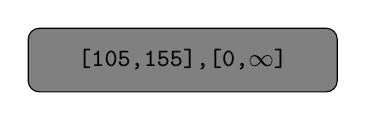
\begin{tikzpicture}
	\node [block4,fill = gray] (n2) {{\tt\small [105,155],[0,$\infty$]}};
	\end{tikzpicture}
}}
&\multirow{2}{*}{9\%}&\multirow{2}{*}{1} 
&                                     \\
&&\multicolumn{1}{c|}{}&\multicolumn{1}{c|}{}  &\multicolumn{1}{c|}{}&\multicolumn{1}{c|}{}
\\
                                                &                        &
\multirow{2}{*}{
\resizebox{0.5\columnwidth}{!}{
	\begin{tikzpicture}
	\node [block3] (n2) {{\tt\small [0,$\infty$],[0,61]}};
	\node [block4,fill = gray,right = 0.3cm of n2] (n3) {{\tt\small [60,76],[0,61]}};
	\node [block3,right = 0.3cm of n3] (n4) {{\tt\small [0,22],[0,$\infty$]}};
	\path [line] (n2) -> (n3);
	\path [line] (n3) -> (n4);
	\end{tikzpicture}
}}
& \multirow{2}{*}{9\%} &\multirow{2}{*}{0.5}                                          &                                     \\
&&\multicolumn{1}{c|}{}&\multicolumn{1}{c|}{}  &\multicolumn{1}{c|}{}&\multicolumn{1}{c|}{}
\\
                                                &                        &
\multirow{2}{*}{
\resizebox{0.5\columnwidth}{!}{
	\begin{tikzpicture}
	\node [block3] (n2) {{\tt\small [0,$\infty$],[29,61]}};
	\node [block4,fill = gray,right = 0.3cm of n2] (n3) {{\tt\small [171,228],[0,$\infty$]}};
	\node [block3,right = 0.3cm of n3] (n4) {{\tt\small [0,46],[0,$\infty$]}};
	\path [line] (n2) -> (n3);
	\path [line] (n3) -> (n4);
	\end{tikzpicture}
}}
&\multirow{2}{*}{4\%} &\multirow{2}{*}{1}                                       &                                     \\
&&\multicolumn{1}{c|}{}&\multicolumn{1}{c|}{}  &\multicolumn{1}{c|}{}&\multicolumn{1}{c|}{}
\\
                                                &                        &
\multirow{2}{*}{
\resizebox{0.18\columnwidth}{!}{
	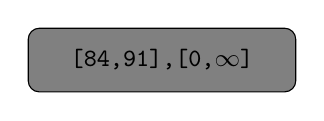
\begin{tikzpicture}
	\node [block3,fill = gray] (n2) {{\tt\small [84,91],[0,$\infty$]}};
	\end{tikzpicture}
}}
& \multirow{2}{*}{4\%} & \multirow{2}{*}{0.5}                                      &                                     \\
&&\multicolumn{1}{c|}{}&\multicolumn{1}{c|}{}  &\multicolumn{1}{c|}{}&\multicolumn{1}{c|}{}
\\
\cline{2-6}
 & \multirow{10}{*}{\rotatebox[origin=c]{90}{2obj}}  &
\multirow{2}{*}{
\resizebox{0.17\columnwidth}{!}{
	\begin{tikzpicture}
	\node [block3,fill = gray] (n2) {{\tt\small [0,$\infty$],[53,61]}};
	\node [None ,above = 0.0cm of n2] (None) {};
	\end{tikzpicture}
}}
& \multirow{2}{*}{9\%} & \multirow{2}{*}{0.53}
& \multirow{10}{*}{
\resizebox{0.15\columnwidth}{!}{
			\begin{tikzpicture}
			\node [None] (n1) {};
			\node [shape=circle,fill=gray,draw=black,below = 0.9cm
                        of n1] (n2) {{\tt n1}};
			\node [None,right = 0.3cm
                        of n1] (n3) {};
			\node [None,above left = 0.7 and 0.5cm
                        of n2] (d1) {};
			\node [None, right = -0.1
                        of d1] (d2) {};
			\node [None, right = -0.1
                        of d2] (d3) {};
			\node [None, right = -0.1
                        of d3] (d4) {};
			\node [None, right = -0.1
                        of d4] (d5) {};
			\node [None, right = -0.1
                        of d5] (d6) {};
			\node [None, right = -0.1
                        of d6] (d7) {};
			\node [None, right = -0.1
                        of d7] (d8) {};
			\node [None, right = -0.1
                        of d8] (d9) {};
			\node [None, right = -0.1
                        of d9] (d10) {};
			\node [None, right = -0.1
                        of d10] (d11) {};
			\node [None, right = -0.1
                        of d11] (d12) {};
			\node [None, right = -0.1
                        of d12] (d13) {};
			\node [None,below left = 0.9 and 0.7cm
                        of n2] (e1) {};
			\node [None, right = -0.1
                        of e1] (e2) {};
			\node [None, right = -0.1
                        of e2] (e3) {};
			\node [None, right = -0.1
                        of e3] (e4) {};
			\node [None, right = -0.1
                        of e4] (e5) {};
			\node [None, right = -0.1
                        of e5] (e6) {};
			\node [None, right = -0.1
                        of e6] (e7) {};
			\node [None, right = -0.1
                        of e7] (e8) {};
			\node [None, right = -0.1
                        of e8] (e9) {};
			\node [None, right = -0.1
                        of e9] (e10) {};
			\node [None, right = -0.1
                        of e10] (e11) {};
			\node [None, right = -0.1
                        of e11] (e12) {};
			\node [None, right = -0.1
                        of e12] (e13) {};
			\node [None, right = -0.1
                        of e13] (e14) {};
			\node [None, right = -0.1
                        of e14] (e15) {};			
			\path [line] (n1) -- (n2);
%			\path [line] (n2) -- (e1);
			\path [line] (n2) -- (e2);
			\path [line] (n2) -- (e3);
			\path [line] (n2) -- (e4);
			\path [line] (n2) -- (e5);
			\path [line] (n2) -- (e6);
			\path [line] (n2) -- (e7);
			\path [line] (n2) -- (e8);
			\path [line] (n2) -- (e9);
			\path [line] (n2) -- (e10);
			\path [line] (n2) -- (e11);
			\path [line] (n2) -- (e12);
			\path [line] (n2) -- (e13);
			\path [line] (n2) -- (e14);
%			\path [line] (n2) -- (e15);
			\end{tikzpicture}
		}
}                   \\
&&\multicolumn{1}{c|}{}&\multicolumn{1}{c|}{}  &\multicolumn{1}{c|}{}&\multicolumn{1}{c|}{}
\\
                                                &
                                                                        &
\multirow{2}{*}{
\resizebox{0.17\columnwidth}{!}{
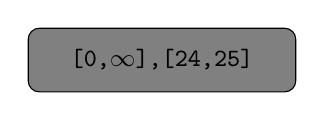
\begin{tikzpicture}
\node [block3,fill = gray] (n2) {{\tt\small [0,$\infty$],[24,25]}};
\end{tikzpicture}
}}
&\multirow{2}{*}{6\%} &\multirow{2}{*}{0.53}                                       &                                     \\
&&\multicolumn{1}{c|}{}&\multicolumn{1}{c|}{}  &\multicolumn{1}{c|}{}&\multicolumn{1}{c|}{}
\\
                                                &                        &
\multirow{2}{*}{\resizebox{0.5\columnwidth}{!}{
	\begin{tikzpicture}
	\node [block4,fill = gray] (n2) {{\tt\small [0,$\infty$],[0,7]}};
	\node [block3,right = 0.3cm of n2] (n3) {{\tt\small [9,11],[0,$\infty$]}};
	\node [block3,right = 0.3cm of n3] (n4) {{\tt\small [76,$\infty$],[0,$\infty$]}};
	\path [line] (n2) -> (n3);
	\path [line] (n3) -> (n4);
	\end{tikzpicture}
}}
&\multirow{2}{*}{2\%}&\multirow{2}{*}{0.82}                                        & \\
&&\multicolumn{1}{c|}{}&\multicolumn{1}{c|}{}  &\multicolumn{1}{c|}{}&\multicolumn{1}{c|}{}
\\

                                                &                        &
\multirow{2}{*}{\resizebox{0.5\columnwidth}{!}{
	\begin{tikzpicture}
	\node [block4] (n2) {{\tt\small [0,$\infty$],[43,$\infty$]}};
	\node [block3,fill = gray,right = 0.3cm of n2] (n3) {{\tt\small [0,$\infty$],[0,14]}};
	\node [block3,right = 0.3cm of n3] (n4) {{\tt\small [22,24],[0,$\infty$]}};
	\path [line] (n2) -> (n3);
	\path [line] (n3) -> (n4);
	\end{tikzpicture}
}}
&\multirow{2}{*}{1\%}&\multirow{2}{*}{0.63}                                        &                                     \\
&&\multicolumn{1}{c|}{}&\multicolumn{1}{c|}{}  &\multicolumn{1}{c|}{}&\multicolumn{1}{c|}{}
\\
                                                &
                                                                        &
\multirow{2}{*}{\resizebox{0.5\columnwidth}{!}{
	\begin{tikzpicture}
	\node [block4] (n2) {{\tt\small [0,$\infty$],[145,147]}};
	\node [block3,fill = gray,right = 0.3cm of n2] (n3) {{\tt\small [0,$\infty$],[0,$\infty$]}};
	\node [block3,right = 0.3cm of n3] (n4) {{\tt\small [0,46],[0,$\infty$]}};
	\path [line] (n2) -> (n3);
	\path [line] (n3) -> (n4);
	\end{tikzpicture}
}}                                                                                &\multirow{2}{*}{1\%}&\multirow{2}{*}{0.69}&                                     \\
&&\multicolumn{1}{c|}{}&\multicolumn{1}{c|}{}  &\multicolumn{1}{c|}{}&\multicolumn{1}{c|}{}
\\

%                                                &                        &
%\resizebox{0.45\columnwidth}{!}{
%	\begin{tikzpicture}
%	\node [block3,fill = gray] (n2) {{\tt\small [0,$\infty$],[0,3]}};
%	\node [block4,right = 0.8cm of n2] (n3) {{\tt\small [22,33],[0,$\infty$]}};
%	\path [line] (n2) -> (n3);
%	\end{tikzpicture}
%}                                       &                                     \\
 \midrule\midrule
\multicolumn{2}{|c|}{\multirow{10}{*}{
		\rotatebox[origin=c]{90}{\makecell{Heap Abstraction\\Heuristic}}}}        &
\multirow{2}{*}{\resizebox{0.5\columnwidth}{!}{
	\begin{tikzpicture}
	\node [block3,fill = gray] (n2) {{\tt\small [0,$\infty$],[0,3]}};
	\node [block4,right = 0.3cm of n2] (n3) {{\tt\small [48,$\infty$],[0,$\infty$]}};
	\node [block4,right = 0.3cm of n3] (n4) {{\tt\small [0,$\infty$],[140,$\infty$]}};
	\path [line] (n2) -> (n3);
	\path [line] (n3) -> (n4);
	\end{tikzpicture}
}}
& \multirow{2}{*}{35\%} &\multirow{2}{*}{0.61} 

& \multirow{10}{*}{
		\resizebox{0.15\columnwidth}{!}{
			\begin{tikzpicture}
			\node [shape=circle,fill = gray,draw=black] (n1) {{\tt
                            n1}};
			\node [shape=circle,draw=black,below = 0.6cm
                        of n1] (n2) {{\tt n2}};
			\node [shape=circle,draw=black,below = 0.6cm
                        of n2] (n4) {{\tt n3}};
			\node [None,right = 0.3cm
                        of n1] (n3) {};
			\node [None,above left = 0.5 and 0.5cm
                        of n2] (d1) {};
			\node [None, right = -0.1
                        of d1] (d2) {};
			\node [None, right = -0.1
                        of d2] (d3) {};
			\node [None, right = -0.1
                        of d3] (d4) {};
			\node [None, right = -0.1
                        of d4] (d5) {};
			\node [None, right = -0.1
                        of d5] (d6) {};
			\node [None, right = -0.1
                        of d6] (d7) {};
			\node [None, right = -0.1
                        of d7] (d8) {};
			\node [None, right = -0.1
                        of d8] (d9) {};
			\node [None, right = -0.1
                        of d9] (d10) {};
			\node [None, right = -0.1
                        of d10] (d11) {};
			\node [None, right = -0.1
                        of d11] (d12) {};
			\node [None, right = -0.1
                        of d12] (d13) {};
			\node [None,below left = 0.4 and 0.7cm
                        of n2] (e1) {};
			\node [None, right = -0.1
                        of e1] (e2) {};
			\node [None, right = -0.1
                        of e2] (e3) {};
			\node [None, right = -0.1
                        of e3] (e4) {};
			\node [None, right = -0.1
                        of e4] (e5) {};
			\node [None, right = -0.1
                        of e5] (e6) {};
			\node [None, right = -0.1
                        of e6] (e7) {};
			\node [None, right = -0.1
                        of e7] (e8) {};
			\node [None, right = -0.1
                        of e8] (e9) {};
			\node [None, right = -0.1
                        of e9] (e10) {};
			\node [None, right = -0.1
                        of e10] (e11) {};
			\node [None, right = -0.1
                        of e11] (e12) {};
			\node [None, right = -0.1
                        of e12] (e13) {};
			\node [None, right = -0.1
                        of e13] (e14) {};
			\node [None, right = -0.1
                        of e14] (e15) {};	
			\node [None,above left = 0.3 and 0.5cm
                        of n4] (1d1) {};
			\node [None, right = -0.1
                        of 1d1] (1d2) {};
			\node [None, right = -0.1
                        of 1d2] (1d3) {};
			\node [None, right = -0.1
                        of 1d3] (1d4) {};
			\node [None, right = -0.1
                        of 1d4] (1d5) {};
			\node [None, right = -0.1
                        of 1d5] (1d6) {};
			\node [None, right = -0.1
                        of 1d6] (1d7) {};
			\node [None, right = -0.1
                        of 1d7] (1d8) {};
			\node [None, right = -0.1
                        of 1d8] (1d9) {};
			\node [None, right = -0.1
                        of 1d9] (1d10) {};
			\node [None, right = -0.1
                        of 1d10] (1d11) {};
			\node [None, right = -0.1
                        of 1d11] (1d12) {};
			\node [None, right = -0.1
                        of 1d12] (1d13) {};
			\node [None,below left = 0.5 and 0.7cm
                        of n4] (1e1) {};
			\node [None, right = -0.1
                        of 1e1] (1e2) {};
			\node [None, right = -0.1
                        of 1e2] (1e3) {};
			\node [None, right = -0.1
                        of 1e3] (1e4) {};
			\node [None, right = -0.1
                        of 1e4] (1e5) {};
			\node [None, right = -0.1
                        of 1e5] (1e6) {};
			\node [None, right = -0.1
                        of 1e6] (1e7) {};
			\node [None, right = -0.1
                        of 1e7] (1e8) {};
			\node [None, right = -0.1
                        of 1e8] (1e9) {};
			\node [None, right = -0.1
                        of 1e9] (1e10) {};
			\node [None, right = -0.1
                        of 1e10] (1e11) {};
			\node [None, right = -0.1
                        of 1e11] (1e12) {};
			\node [None, right = -0.1
                        of 1e12] (1e13) {};
			\node [None, right = -0.1
                        of 1e13] (1e14) {};
			\node [None, right = -0.1
                        of 1e14] (1e15) {};				
			\path [line] (n1) -- (n2);
			\path [line] (n1) -- (n3);
			\path [line] (d1) -- (n2);
			\path [line] (d2) -- (n2);
			\path [line] (d3) -- (n2);
			\path [line] (d4) -- (n2);
			\path [line] (d5) -- (n2);
			\path [line] (d6) -- (n2);
			\path [line] (d7) -- (n2);
			\path [line] (d8) -- (n2);
			\path [line] (d9) -- (n2);
			\path [line] (d10) -- (n2);
			\path [line] (d11) -- (n2);
			\path [line] (d12) -- (n2);
			\path [line] (d13) -- (n2);
%			\path [line] (n2) -- (e1);
			\path [line] (n2) -- (e2);
			\path [line] (n2) -- (e3);
			\path [line] (n2) -- (e4);
			\path [line] (n2) -- (e5);
			\path [line] (n2) -- (e6);
			\path [line] (n2) -- (e7);
			\path [line] (n2) -- (e8);
			\path [line] (n2) -- (e9);
			\path [line] (n2) -- (e10);
			\path [line] (n2) -- (e11);
			\path [line] (n2) -- (e12);
			\path [line] (n2) -- (e13);
			\path [line] (n2) -- (e14);
%			\path [line] (n2) -- (e15);
			\path [line] (n2) -- (n4);
			\path [line] (1d1) -- (n4);
			\path [line] (1d2) -- (n4);
			\path [line] (1d3) -- (n4);
			\path [line] (1d4) -- (n4);
			\path [line] (1d5) -- (n4);
			\path [line] (1d6) -- (n4);
			\path [line] (1d7) -- (n4);
			\path [line] (1d8) -- (n4);
			\path [line] (1d9) -- (n4);
			\path [line] (1d10) -- (n4);
			\path [line] (1d11) -- (n4);
			\path [line] (1d12) -- (n4);
			\path [line] (1d13) -- (n4);
%			\path [line] (n4) -- (1e1);
			\path [line] (n4) -- (1e2);
			\path [line] (n4) -- (1e3);
			\path [line] (n4) -- (1e4);
			\path [line] (n4) -- (1e5);
			\path [line] (n4) -- (1e6);
			\path [line] (n4) -- (1e7);
			\path [line] (n4) -- (1e8);
			\path [line] (n4) -- (1e9);
			\path [line] (n4) -- (1e10);
			\path [line] (n4) -- (1e11);
			\path [line] (n4) -- (1e12);
			\path [line] (n4) -- (1e13);
			\path [line] (n4) -- (1e14);
%			\path [line] (n4) -- (1e15);
			\end{tikzpicture}
		}
}\\
\multicolumn{1}{|c}{}&\multicolumn{1}{c|}{}&\multicolumn{1}{c|}{}&\multicolumn{1}{c|}{}  &\multicolumn{1}{c|}{}&\multicolumn{1}{c|}{}
\\
\multicolumn{2}{|l|}{}                                                   &
\multirow{2}{*}{\resizebox{0.5\columnwidth}{!}{
	\begin{tikzpicture}
	\node [block3,fill = gray] (n2) {{\tt\small [0,12],[0,3]}};
	\node [block4,right = 0.3cm of n2] (n3) {{\tt\small [0,97],[0,$\infty$]}};
	\node [block4,right = 0.3cm of n3] (n4) {{\tt\small [0,$\infty$],[140,$\infty$]}};
	\path [line] (n2) -> (n3);
	\path [line] (n3) -> (n4);
	\end{tikzpicture}
}}
&\multirow{2}{*}{33\%}
&\multirow{2}{*}{0.53}                                      &                                     \\
\multicolumn{1}{|c}{}&\multicolumn{1}{c|}{}&\multicolumn{1}{c|}{}&\multicolumn{1}{c|}{}  &\multicolumn{1}{c|}{}&\multicolumn{1}{c|}{}
\\
\multicolumn{2}{|l|}{}                                                   &
\multirow{2}{*}{\resizebox{0.40\columnwidth}{!}{
	\begin{tikzpicture}
	\node [block4,fill = gray] (n3) {{\tt\small [38,$\infty$],[0,62]}};
	\node [block4,right = 0.8cm of n3] (n4) {{\tt\small [0,$\infty$],[236,$\infty$]}};
	\path [line] (n3) -> (n4);
	\end{tikzpicture}
}}
& \multirow{2}{*}{27\%} &\multirow{2}{*}{0.59}                                        &                                     \\
\multicolumn{1}{|c}{}&\multicolumn{1}{c|}{}&\multicolumn{1}{c|}{}&\multicolumn{1}{c|}{}  &\multicolumn{1}{c|}{}&\multicolumn{1}{c|}{}
\\
\multicolumn{2}{|l|}{}                                                   &
\multirow{2}{*}{\resizebox{0.40\columnwidth}{!}{
	\begin{tikzpicture}
	\node [block4,fill = gray] (n3) {{\tt\small [0,48],[0,62]}};
	\node [block4,right = 0.8cm of n3] (n4) {{\tt\small [72,84],[0,$\infty$]}};
	\path [line] (n3) -> (n4);
	\end{tikzpicture}
}}
& \multirow{2}{*}{24\%} & \multirow{2}{*}{0.53} 
                                         &\\
\multicolumn{1}{|c}{}&\multicolumn{1}{c|}{}&\multicolumn{1}{c|}{}&\multicolumn{1}{c|}{}  &\multicolumn{1}{c|}{}&\multicolumn{1}{c|}{}
\\
\multicolumn{2}{|l|}{}                                                   &
\multirow{2}{*}{\resizebox{0.5\columnwidth}{!}{
	\begin{tikzpicture}
	\node [block3,fill = gray] (n2) {{\tt\small [0,24],[0,$\infty$]}};
	\node [block4,right = 0.3cm of n2] (n3) {{\tt\small [21,$\infty$],[140,$\infty$]}};
	\node [block4,right = 0.3cm of n3] (n4) {{\tt\small [0,97],[0,$\infty$]}};
	\path [line] (n2) -> (n3);
	\path [line] (n3) -> (n4);
	\end{tikzpicture}
}}
& \multirow{2}{*}{22\%} & \multirow{2}{*}{0.53} 
                                         &                                     \\
\multicolumn{1}{|c}{}&\multicolumn{1}{c|}{}&\multicolumn{1}{c|}{}&\multicolumn{1}{c|}{}  &\multicolumn{1}{c|}{}&\multicolumn{1}{c|}{}
\\
%\multicolumn{2}{|l|}{}                                                   &
%\resizebox{0.45\columnwidth}{!}{
%	\begin{tikzpicture}
%	\node [block3,fill = gray] (n2) {{\tt\small [0,48],[0,$\infty$]}};
%	\node [block4,right = 0.8cm of n2] (n3) {{\tt\small [72,84],[0,$\infty$]}};
%
%	\path [line] (n2) -> (n3);
%	\end{tikzpicture}
%}                                         &                                     \\
\bottomrule
\end{tabular}
\caption{Top-5 features learned by our technique, and concrete nodes implied by the top-1 feature.
%Gray colored abstract nodes in the features correspond to the target nodes and others are predecessors or successors.
%Gray colored nodes in the column \textsf{Concretization} are precision-critical nodes which are selected by the first features; 
%other nodes are predecessors or successors that make the gray colored nodes satisfy the features.
}
\label{fig:features}
\end{figure}



%%% Local Variables:
%%% mode: latex
%%% TeX-master: "paper"
%%% End:


\myparagraph{Top-5 Features}
Figure~\ref{fig:features} describes the most informative features generated by our technique for each abstraction degree and their concretization in the given graphs.
The second column \textsf{Top 5 Features}, in decreasing order of \textsf{portion}, presents top 5 features which have the greatest number of precision-critical nodes satisfying the features with scores above 0.5.
For example, the first feature in 1type contains 47\% nodes of the total precision-critical nodes which are to be applied 1-type-sensitivity,
and has a score of 0.57.
If a feature is too general (e.g., $(\epsilon, ([0,\infty],[0,\infty]), \epsilon)$), it is excluded even with a large portion (e.g., 100\%)
because its score is under 0.5.
Similarly, if a feature is too specific, it is also excluded because it includes a small number of precision-critical nodes even with a good score.
For the features, the gray colored abstract nodes correspond to the target one $\hat{n}$ in each feature
(e.g., $(\seq{\myhat{p}_0,\myhat{p}_1,\dots,\myhat{p}_q}, \myhat{n}, \seq{\myhat{s}_0,\myhat{s}_1,\dots,\myhat{s}_r}) \in \Feature$).
Other nodes are predecessors or successors of the target abstract nodes (e.g., $\myhat{p}_0$, $\myhat{s}_0$, and $\myhat{s}_1$).
For each feature, we show the number of satisfying nodes over the total precision-critical nodes in the given graphs (\textsf{portion}) and the scores (\textsf{score}).
The right most column, \textsf{Concretization}, illustrates the visualized concretization for each first feature in \textsf{Top 5 Features} column,
%in the real graphs over the training programs, where the gray colored nodes correspond to the target nodes of the first feature.
where the gray colored nodes correspond to the target abstract nodes of the first feature.
For space reasons, we draw each node to have at most 13 incoming and outgoing edges although it can have more than 13 edges.


\begin{table}[]
\setlength\extrarowheight{-1pt}
\caption{Performance of our manually-designed graph-based heap abstraction heuristic for FPG}
\label{tbl:principle}
\centering
\footnotesize
\begin{tabular}{@{}clrr | clrr@{}}
\toprule
benchmarks               & \multicolumn{1}{c}{} & \multicolumn{1}{c}{alarms} & \multicolumn{1}{c|}{time(s)} & benchmarks                & \multicolumn{1}{c}{} & \multicolumn{1}{c}{alarms} & \multicolumn{1}{c}{time(s)} \\ \midrule
\multirow{2}{*}{luindex} & \Principle              & 374                        & 29(+29)                         & \multirow{2}{*}{lusearch} & \Principle            & 388                        & 33(+31)                        \\
                         % & \OurHeap            & 358                        & 23                          &                           & \OurHeap              & 372                        & 21                          \\
                         & \AllocBased          & 358                        & 5,475                       &                           & \AllocBased          & -                          & $>$10,800        \\\midrule
\multirow{2}{*}{antlr}   & \Principle              & 478                        & 44(+47)                        & \multirow{2}{*}{pmd$_{m}$}      & \Principle            & 886                        & 83(+65)                          \\
                         % & \OurHeap            & 463                        & 49                          &                           & \OurHeap              & 871                        & 48                          \\
                         & \AllocBased          & 463                        & 5,241                       &                           & \AllocBased          & 871                        & 9,146                       \\\midrule
\multirow{2}{*}{fop}     & \Principle            & 391                        & 41(+46)                          & \multirow{2}{*}{xalan}    & \Principle            & 548                        & 841(+85)                         \\
                         % & \OurHeap              & 376                        & 30                          &                           & \OurHeap              & 539                        & 489                         \\
                         & \AllocBased          & -                          & $>$10,800        &                           & \AllocBased          & -                          & $>$10,800        \\ \bottomrule
\end{tabular}
\end{table}


\myparagraph{Insights}

The generated features during the learning process provide hints on designing analysis heuristics from the graphs.
For example, we investigated the features of the heap abstraction heuristic in Figure~\ref{fig:features} and found two commonalities in them.
First,  the features have the form of $(\epsilon,\hat{n}, \hat{\vec{s}})$ where $\hat{\vec{s}}$ is not $\epsilon$,
which implies that we should consider successors more than predecessors when designing heap abstraction heuristics from points-to graph.
The second commonality is that $\hat{\vec{s}}$ or $\hat{n}$ tends to include an abstract
node $\aNode$ that presents nodes with lots of outgoing edges, i.e., $\aNode =
(itv,[b,\infty])$ where the number $b$ is about $3\%$ of the total nodes in a graph of a training program.
From these observations, we manually designed a graph-based heap abstraction heuristic which
assigns allocation-site based heap abstraction to the target nodes
if at least $3\%$ of the total nodes in FPG belong to either the target node or its successor nodes
(i.e. $\heuristic = \seq{\{ (\epsilon,([0,\infty],[b',\infty]),\epsilon)
	,(\epsilon,\top,\seq{([0,\infty],[b',\infty])})
	,(\epsilon,\top,\seq{\top,([0,\infty],[b',\infty])})
	,\dots
	\}
}$ where $\top$ equals to the most general one $([0,\infty],[0,\infty])$ and $b'$ is 3\% of the total nodes in the given graph).
Otherwise, the heuristic assigns type-based heap abstraction to the others.
%where $\top$ equals to the most general abstract node $([0,\infty],[0,\infty])$, and $b$ equals to 3\% of the total nodes in the given graph).
Table~\ref{tbl:principle} demonstrates the performance of the manually-crafted heuristic.
In comparison to \AllocBased, it reduces about 99\% of analysis cost while producing only 2\% more alarms.
%Compared to the baseline heuristic~\AllocBased,



Intuitively, the nodes with lots of successors in FPG should be analyzed precisely because merging the objects with others would produce lots of spurious analysis results.
For example, if there exists an object with lots of field objects which we want to merge with another one with a few field objects,
it eventually produces lots of spurious results stating that the both heaps can have lots of field objects.
%Such insight is related with that of \Mahjong~which merges the two objects if they have the same types of successors because,
%statically, an object having lots of successors is hard to have exactly the same types of successors with other objects.
Such insight is related with that of \Mahjong~which merges the objects if their successors have the same type;
statistically, if an object has lots of successors, there hardly exist the other objects with exactly the same types of successors.
Surprisingly, it is easy to find such insight through the features generated by our technique.
Note that this insight is general as it is not dependent to Java programs.
For example, when analyzing a C program, it is a required task not to merge such heaps with others as it would produce lots of spurious results.

%\textcolor{black}{
%\myparagraph{Graphick vs Scaler}
%Interestingly, Figure~\ref{fig:features} shows that the insight learned statistically can differ from the logic-based insight
%through the difference between \OurCtx~and \Scaler~in deciding which nodes to analyze more precisely.
Interestingly, Figure~\ref{fig:features} also shows the difference between the statistically-learned insight behind \OurCtx~and the logical insight behind \Scaler~in deciding which nodes to analyze more precisely.
Based on the logical insight, \Scaler~relies heavily on the number of incoming edges
as that number in the object allocation graph indicates %{\color{red}{
how many contexts will be constructed in object sensitivity.%}}
~\ourtool, however, treats the number of neighbor nodes' outgoing edges more importantly, as shown in Figure 6.
Such differences result in the performance gap between the two object-sensitivity heuristics.
%which shows better performance in both precision and scalability than the logic-based insight.
%}

%\textcolor{red}{
\myparagraph{Generality of learned heuristic}
We found the learned heuristic for object sensitivity is general to the hybrid-context sensitivity~\cite{KastrinisS13a}. Table~\ref{tbl:hybrid} presents the performance of the conventional 2-hybrid-context sensitivity (\twosobjH) and
2-hybrid-context sensitivity with the learned heuristic (\ourtool) used in Section~\ref{sec:comparescaler}.
%when using 6 DaCapo benchmark programs as testing programs.
The table shows that \ourtool~is also cost-effective compared to \twosobjH. For example, on a test program bloat,
\ourtool~produces only 22 more alarms while reducing about 90\% of analysis costs.
%}



\begin{table}[]
\setlength\extrarowheight{-1pt}
\caption{Performance comparison between conventional 2-hybrid-context-sensitivity (\twosobjH) and 2-hybrid-context-sensitivity with our learned heuristic for 2-object-sensitivity (\ourtool).}
\label{tbl:hybrid}
\centering\footnotesize
\begin{tabular}{@{}clrrrrrr@{}}
\toprule
                          & \multicolumn{1}{c}{} & \multicolumn{1}{c}{pmd$_m$} & \multicolumn{1}{c}{chart} & \multicolumn{1}{c}{eclipse} & \multicolumn{1}{c}{xalan} & \multicolumn{1}{c}{fop} & \multicolumn{1}{c}{bloat}  \\ \midrule
\multirow{2}{*}{\ourtool} & \#may-fail casts     & 220                      & 867                       & 2,880                        & 479                       & 1,408                    & 1,147                      \\
                          & analysis time (s)    & 45+(78)                  & 83(+76)                   & 1,426(+105)                  & 185(+57)                  & 245(+85)                & 215(+30)                  \\ \midrule
\multirow{2}{*}{\twosobjH}    & \#may-fail casts     & 220                      & 757                       & -                       & 447                          &  1,295                       & 1,125                          \\
                          & analysis time (s)    & 42                       & 195                       & $>$ 10,800                            & 428                          & 818                        & 2,238                           \\
%\midrule
%\multirow{2}{*}{\Insens}   & \#may-fail casts     & 679                      & 1,810                      & 4190                        & 1,182                      & 2,458                    & 1,924                      \\
%                          & analysis time (s)    & 23                       & 48                        & 91                          & 37                        & 53                      & 20                        \\
\bottomrule
\end{tabular}
\end{table}




%%% Local Variables:
%%% mode: latex
%%% TeX-master: "paper"
%%% End:

% !TEX root = ./paper.tex

\subsection{Performance Variations on Different Training Datasets}\label{sec:justify}

We constructed a benchmark suite with the programs from the DaCapo suite,
and used 3$\sim$4 small programs (i.e. luindex, lusearch, antlr, and pmd$_{m}$) as our training set.
In this subsection, we evaluate \ourtool~on different combinations of training data to see how its performance is affected by the number of training programs.

%Despite the small number and small size, they provide sufficient information to learn cost-effective heuristics,
%and we conducted an additional experiment to justify this evaluation setting.


We found that the amount of training data is overall critical, and
using four small programs as a training set can produce competitive heap abstraction heuristics cost-effectively.
Table~\ref{tbl:training} presents the performance and scores
(i.e. ${\mbox{\#proven casts}}\over{\mbox{analysis time (s)}}$)
of each heuristic learned with various combinations of training programs (i.e., \onepgm, \twopgm, \threepgm, and \fourpgm) and an ideal heuristic (\ideal) against the validation program findbugs.
For the ideal heuristic (\ideal), we assume that it has the precision of \Mahjong~and the scalability of \TypeBased~
since they are the most precise and the most scalable respectively in our space of heap abstraction heuristic.
The second row, analysis time (s), in table~\ref{tbl:training} indicates the amount of time each heuristic took to successfully analyze the validation program, and
the third row, \#proven casts, presents the number of castings proved to be safe;
thereby, the more precise the analysis, the greater the number of proven casts.
As shown in Table~\ref{tbl:training}, the score increases with respect to the size of training set.
The score of \fourpgm~(i.e. 13.6) is nearly the same with that of the ideal heuristic (i.e. 15.4) in our evaluation.
It implies that using four programs as a training set is sufficient to produce cost-effective heap abstraction heuristics.


% among the various combinations of our training programs.
%In Table~\ref{tbl:training}, \onepgm, \twopgm, \threepgm, and \fourpgm correspond to the heuristics learned with
%{\it npgm} $(1 \le n\le 4)$ indicates the number of training programs used for learning heuristics.
%We calculate the cost of the ideal heuristic with the cost of \TypeBased~and the proven queries by \Mahjong~
%because \TypeBased~is most scalable
%and \Mahjong~is most precise in our space of heap abstraction heuristics.
%
%
%The row score present the quality of the learned heuristics and an ideal heuristic
%
%The black solid line and red dotted line in the graph present the scores of our learned heuristics and an ideal heuristic (i.e.,
%${\small {\mbox{proven queries in \Mahjong}}\over{
%\mbox{cost of \TypeBased}}}$),
%respectively.
%We calculate the cost of the ideal heuristic with the cost of \TypeBased~and the proven queries by \Mahjong~
%because \TypeBased~is most scalable
%and \Mahjong~is most precise in our space of heap abstraction heuristics.
%\minseok{revision}

%In our experiments, we used 3 $\sim$ 4 programs for our training set.

%\textcolor{red}{
%Although we used a small number of small programs (e.g., luindex, lusearch, antlr, pmd$_{m}$) as a training set, those training programs do not represent unrealistic training data.

Using four programs as training programs could produce cost-effective heuristics because, even though our training programs are the smallest among the total benchmark programs,
they still provide sufficient learning data for our approach.
First, the DaCapo suite itself is a collection of realistic programs.
DaCapo has been carefully designed to include various behaviors and complex codes~\cite{Blackburn2006}.
For example, even the smallest program (i.e. lusearch) in Dacapo has more methods than the largest one in the SPEC benchmark~\cite{specjvm98}.
Secondly, when training heuristics in our approach, what matters is the number of allocation-sites, not the number of programs;
the learning algorithm of \OurCtx~treats individual allocation-sites as labelled data.
Our training programs provide sufficient training data to learn cost-effective heuristics in this sense.
%The training programs we used provide sufficient number of learning data.
More precisely, the smallest program (lusearch) has 4,752 allocation-sites,
and the remaining three training programs (lusearch, antlr, pmd$_{m}$) provide 14,068 unique allocation-sites in total;
we have a total of 18,820 allocation-sites for training data.
%}

%\textcolor{red}{
In practice, we recommend a user to choose programs with less than 400 classes as training programs, for which we found Grahpick typically works well. Although limited, our experience shows that a collection of such programs can provide useful training data.
%}
%\begin{table}[]
%\small
%\caption{Performance comparison among heuristics learned with various numbers (1$\sim$4) of training programs.}
%\label{tbl:training_pgms}
%\begin{tabular}{@{}clrrrr@{}}
%\toprule
%         & \multicolumn{1}{c}{} & \multicolumn{1}{c}{\onepgm} & \multicolumn{1}{c}{\twopgm} & \multicolumn{1}{c}{\threepgm} & \multicolumn{1}{c}{\fourpgm} \\ \midrule
%% \multirow{2}{*}{luindex}  & analysis time (s)    & 26(+27)                   & 41(+26)                   & 23(+50)                   & 23(+90)                   \\
%% %\multirow{2}{*}{luindex}  & analysis time (s)    & 26                   & 41                   & 23                   & 23                   \\
%%          & \#may-fail casts     & 358                       & 358                       & 358                       & 358                       \\ \bottomrule
%%\multirow{2}{*}{findbugs} & analysis time (s)    & 4,090               & 411                 & 153                 & 96                  \\
%\multirow{2}{*}{findbugs} & analysis time (s)    & 4,090(+185)               & 411(+107)                 & 153(+226)                 & 96(+363)                  \\
%         & \#may-fail casts     & 2,417                     & 1,768                      & 1,800                     & 1,774                     \\ \bottomrule
%\end{tabular}
%\end{table}
%
%
%\begin{figure}
%	\centering
%		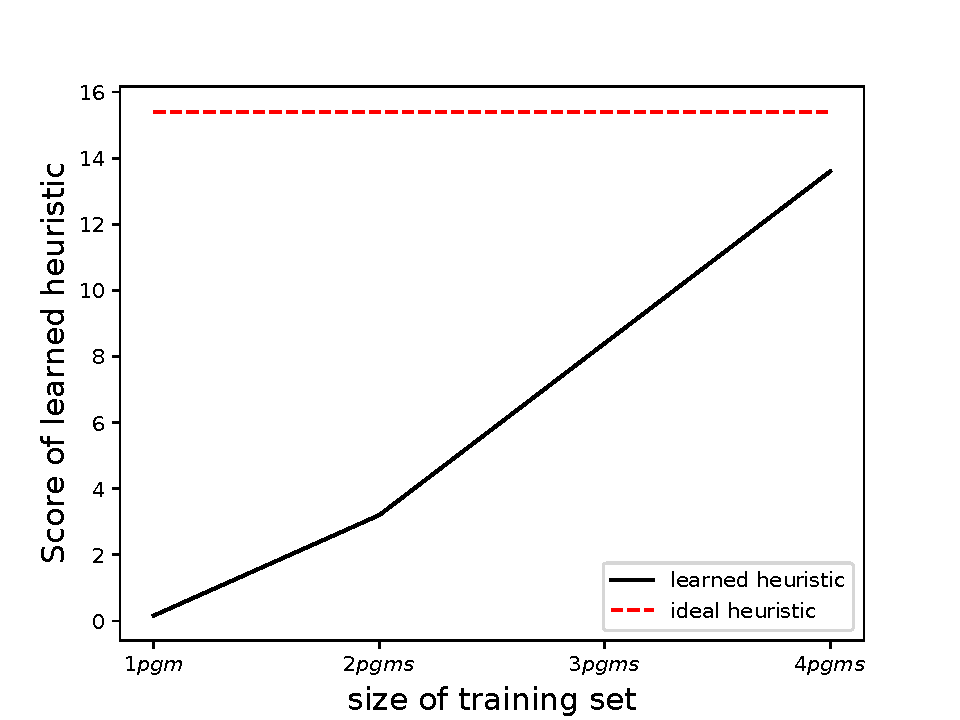
\includegraphics[width=7cm]{figures/training_set.pdf}
%	\caption{How score of learned heuristic changes over the value
%		of $\hyper$.}
%	\label{fig:training}
%\end{figure}


% Please add the following required packages to your document preamble:
% \usepackage{booktabs}
\begin{table}[]
\setlength\extrarowheight{-1pt}
\caption{Performance comparison among heuristics learned from various combinations of training sets (i.e. \onepgm, \twopgm, \threepgm, and \fourpgm) and an ideal heuristic (\ideal) against the validation program findbugs. \#proven casts presents the number of casts proved to be safe; a more precise analysis produces a larger number of \#proven casts.
The row score presents the quality of the heuristics computed by
${\mbox{\#proven casts}}\over{\mbox{analysis time (s)}}$.}
\label{tbl:training}
%${\projproved(F_P(\heuristic(G)))}\over{\projcost(F_P(\heuristic(G)))}$.}
\centering\scriptsize
\begin{tabular}{@{}lrrrrr@{}}
\toprule
%\multicolumn{1}{c}{} & \multicolumn{1}{c}{\onepgm} & \multicolumn{1}{c}{\twopgm} & \multicolumn{1}{c}{\threepgm} & \multicolumn{1}{c}{\fourpgm} & \multicolumn{1}{c}{\multirow{3}{*}{\ideal}} \\
\multicolumn{1}{c}{\multirow{2}{*}{}} & \multirow{2}{*}{\{luindex\}} & \multicolumn{1}{c}{\multirow{2}{*}{\{luindex, lusearch\}}} & \multicolumn{1}{c}{\{luindex, lusearch} & \multicolumn{1}{c}{\{luindex, lusearch} & \multicolumn{1}{c}{\multirow{2}{*}{\qquad\ideal}} \\
\multicolumn{1}{c}{} &  &  & \multicolumn{1}{c}{antlr\}}  & \multicolumn{1}{c}{antlr, pmd\}} &  \\ \midrule
analysis time (s)    & 4,090(+185)                                & 411(+107)                                  & 153(+226)                                    & 96(+363)                                    & 92                        \\
\#proven casts     & 672                                      & 1,321                                      & 1,289                                        & 1,315                                       & 1418                      \\ \midrule
score                & 0.16                   & 3.2                    & 8.4                      & 13.6                    & 15.4 \\\bottomrule
\end{tabular}
\end{table}


%\begin{figure}
%\vspace{-22pt}
%\begin{multicols}{2}
%~\\~\\~\\
%\begin{subfigure}[]{0.9\columnwidth}
%\small
%%\begin{tabular}{@{}c|lrr@{}}
%%\toprule
%%\multicolumn{1}{c}{}                          & \multicolumn{1}{c}{} & \multicolumn{1}{c}{\onepgm}   & \multicolumn{1}{c}{\twopgm}  \\ \midrule
%%\multirow{5}{*}{findbugs} & analysis time (s)    & 4,090(+185)                  & 411(+107)                   \\
%%                          & \#may-fail casts     & 2,417                        & 1,768                       \\ \cmidrule(){2-4}
%% & \multicolumn{1}{c}{} & \multicolumn{1}{c}{\threepgm} & \multicolumn{1}{c}{\fourpgm} \\
%%						  \cmidrule(){2-4}
%%                          & analysis time (s)    & 153(+226)                    & 96(+363)                    \\
%%                          & \#may-fail casts     & 1,800                        & 1,774                      \\\bottomrule
%%\end{tabular}
%\end{subfigure}
%
%\columnbreak
%\vspace{-57pt}
%\begin{subfigure}[t]{0.9\columnwidth}
%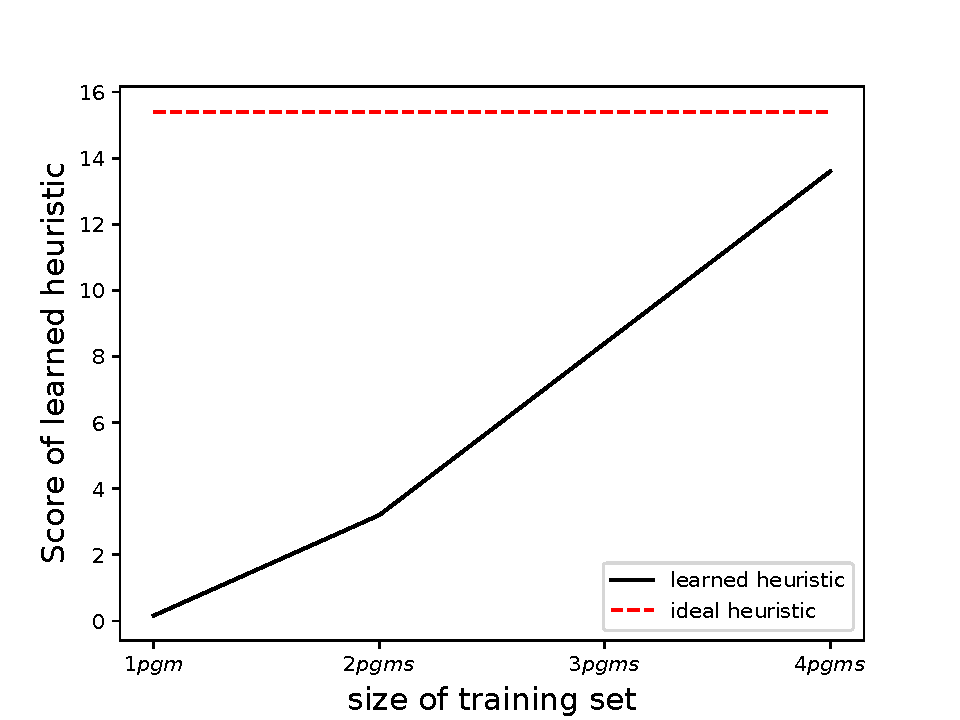
\includegraphics[width=7cm]{figures/training_set.pdf}
%\end{subfigure}
%\end{multicols}
%\vspace{-0.5cm}
%\caption{Performance of heuristics learned with various numbers (1$\sim$4) of training programs, and how score of learned heuristic changes over the size of training set.}
%\label{fig:training}
%\end{figure}

%
%	\centering
%	\begin{tabular}{cc}
%		% Please add the following required packages to your document preamble:
%% \usepackage{booktabs}
%% \usepackage{multirow}
%
%&
%		
%	\end{tabular}
%		of $\hyper$.}
%	\label{fig:gamma}
%






%%% Local Variables:
%%% mode: latex
%%% TeX-master: "paper"
%%% End: 
% !TEX root = ./paper.tex

%\textcolor{red}{
%The heuristics produced by \ourtool~ may not be general when the downstream clients for training steps are substantially different from those in evaluation.
%In experiments, we trained heuristics with the may-fail-cast client and evaluated the learned heuristics on the test set using three clients (may-fail-casts, poly-call-sites, and call-graph-edges).
%The evaluation results show that the heuristics learned by \ourtool~ are general in our evaluation environment.
%The performance, however, may be unsatisfactory if the clients in the main analysis are different from the ones used when training. In such a case, \ourtool~should be retrained with the new target client.
%}




\subsection{Limitations and Discussion}
%\TODO{Explain more about the limitation: e.g., Limitation 1 is ... Limitation 2 is ... And then discuss how to mitigate them in a separate paragraph.}
\ourtool~has several limitations.
One major limitation is that the heuristics produced by our approach may not be generalized
if the setting in training steps is substantially different from that used in evaluation in terms of analyzer $F$, target client, and $\CallDepth$.
More specifically, the learned heuristics by \ourtool~are dependent on the training data, the analyzer $F$ used, and the target client
(e.g., may-fail casts).
For example, the precision on the number of may-fail casts can be unsatisfactory if we train the heuristics with
the number of poly-call sites as the target client.
The context-length $\CallDepth$ for the main analysis is also limited to the one used in the training phase.
%d) the context-length k used in the training phase is rather limited.
Besides those generality issues, the training process of \ourtool~is time-consuming (i.e. it took 200 hours in our evaluation).

%As the heuristics produced by \ourtool~is learned with the a) the training data and b) specific analyzer $F$,
%the performance of \ourtool~may be unsatisfactory if the analyzer for main analysis is different from the one used in training phase.
%Similarly, using different clients for the main analysis from the training process can result in the degraded performance of \ourtool~
%in terms of precision and scalability.
%For example, the precision on the number of may-fail casts can be unsatisfactory if we train the heuristics with
%the number of poly-call sites as the target client.
%Further, e) the learning cost of~\ourtool takes about 200 hours for a single heuristic,
%which seems to be costly.

Despite those limitations, we believe \ourtool~can be useful in practice. %for other settings as well in practice.
First of all, note that in this paper we showed the effectiveness of \ourtool~in a realistic (yet particular) setting, where we used a real-world pointer analysis framework and benchmarks.
In particular, we do not believe the expensive training phase of \ourtool~is a serious limitation in practice, because it is not only fully automatic but also rather cheap compared to the much more expensive process of handcrafting analysis heuristics or features by human experts.
%\ourtool~can automate the manual process that typically requires weeks or months to develop a single heuristic.
%All the processes of generating the heuristics are fully automated, which can dramatically reduce the
%burdens of analysis designers in practice.
%Even with the limitations above,~\ourtool, however, can be still used realistically in a production setting.
%For example, although it takes about 200 hours to learn a single heuristic, it is cheaper than the manual process of
%designing cost-effective heuristics from the given graph, which typically takes weeks or months.
%Moreover, all the processes of generating the heuristics are fully automated, which can dramatically reduce the
%burdens of human-involving tasks.
The learned heuristic is dependent on the training data but, as we showed in this paper (Section~\ref{sec:justify}), using a small number of real programs is likely to provide a sufficient amount of actual training data (e.g., allocation sites) in practice. Also, the selection of training programs did not require careful engineering efforts in our case.
The context length $\CallDepth$ is rather limited (2-object-sensitivity), but 2-object-sensitive pointer analysis is generally considered to be highly precise in practice~\cite{Li2018a}.

For the issue on target clients, we showed that training heuristics using the may-fail-cast client
generalizes well for the three clients (may-fail-casts, poly-call-sites, and call-graph-edges).
When the downstream clients are substantially different, however,
one solution is to choose the target clients as general as possible in the training process. For example, we can use the size of context-insensitive variable points-to sets instead of the number of may-fail-casts as the context-insensitive variable points-to set is one of the most general clients that affect the others.
The clients we used in our evaluation (i.e. may-fail-casts, poly-call-sites, and call-graph-edges) are computed based on the context-insensitive variable points-to set and therefore minimizing it would likely minimize other clients too.
%
%\TODO{What is the point of the next paragraph? Saying another limitation and how to mitigate it? Be more explicit. }
%Despite its dependency on the settings (e.g., training data, analyzer $F$, target client, and context depth $k$) and learning cost,
%\ourtool~can be practically used in industry because user-involving tasks (e.g., deciding suitable settings) are light weighted and other processes are done automatically.
%More precisely, for the analyzer $F$, the users only need to decide the one among the other available analyzers to suit their tastes.
%Users can also organize the training data with other programs which have commonalities to the object program (e.g., functional behavior, type of inputs). These commonalities would likely provide appropriate data for learning.
%For the context depth $k$, the users can simply determine the highest context depth $k$
%by checking whether $\vec{k}$ (assign $k$ to all the program components) is scalable over the training programs while $\vec{k+1}$ (assign $k+1$ to all the program components) is not.
%With the selected settings above, \ourtool~automatically produces the cost-effective heuristics,
%of which the learning process takes about 200 hours.
%Although the learning cost seems to be expensive, we believe that it is reasonably cheaper compared to the cost of manually designing graph-based heuristics which additionally requires high expertise and lots of human effort.
%
%





%As \ourtool~automates the processes which typically require lots of human effort,
%it can reduce the burdens
%it is much more light weighted compared to manually designing graph-based heuristics which additionally requires high expertise and lots of human effort.

%Only with small effort on deciding the settings, \ourtool~automatically produces the cost-effective heuristics.







%\textcolor{blue}{Tone down the claim of Graphick as "an approach to learn heuristics for "object-sensitive" pointer analysis" instead of "a general-purpose approach to context-sensitive pointer analysis". In particular, argue convincingly how GraphicK can be used realistically in a production setting, given that (a) its training phase is time-consuming, (b) the learned predictor is dependent on the training data and the analyser F used, and (3) the context-length k used in the training phase is rather limited.}



%%% Local Variables:
%%% mode: latex
%%% TeX-master: "paper"
%%% End:

%\chapter{Related Work}\label{sec:Related}
%% !TEX root = ./paper.tex

\section{Conclusion and Future Work}

Unfortunately, the program analysis community for object-oriented programs has dismissed call-site sensitivity for a long time. 
In this paper, 
showed that 
call-site sensitivity has vast untapped potential, even more than object sensitivity, when the notion of $k$-limiting is generalized. We provided an insight that call-site sensitivity with context tunneling can simulate object sensitivity and experimentally proved that the observation holds in practice by developing a technique to transform a baseline object-sensitive analysis into more precise, context-tunneled call-site sensitivity. 
Based on our results, we hope that the community reconsiders call-site sensitivity from now on.  


%We demonstrated that our technique enables call-site sensitivity to outperform modern object-sensitive analyses for real-world Java programs in both precision and cost.

%when designing context-sensitive analyses.


Many problems remain as future work. We already discussed a theoretical issue in Section~\ref{sec:counter_example}. 
Other problems include the following. 


\begin{itemize}

\item {\em Can we learn better tunneling strategies than just simulating object sensitivity?} 
Our goal in this paper was to show that call-site sensitivity can be superior to object sensitivity, and simulating object sensitivity was an effective means of achieving this goal. 
However, simulating object sensitivity would be a suboptimal strategy for call-site sensitivity; 
we believe an optimal tunneling strategy would enable call-site sensitivity to show far better precision than ours (\ours).
Thus, an interesting direction for future work is to develop a powerful learning algorithm to find such strategies, where 
the main challenge is how to efficiently explore the huge and non-monotone tunneling space~\cite{JeJeOh18}. Using reinforcement learning, for example, could be a promising approach to address this challenge. 

%in the huge and non-monotone tunneling space~\cite{JeJeOh18}. 
%For example, reinforcement learning could be a promising approach to address this challenge.

\item {\em Can our approach be adapted for other flavors of context-sensitive analyses?}
Our current simulation technique relies on properties specific to $k$-CFA (e.g., $I_2$ in Section~\ref{sec:simulation} leverages a unique property of context-tunneled $k$-CFA). However, the high-level idea (i.e., simulating object sensitivity) would be applicable to other analyses. 
For example, it would be interesting if our idea could be adapted for $m$-CFA~\cite{Might10}. 
% by leveraging properties of context-tunneled $m$-CFA. 



% instead of k-CFA with your technique would produce better, similar, or worse results.


% High-level idea of our approach (simulating object sensitivity) is applicable to other contexts. 
%Directly applying our technique may not effective as
%it relies on specific properties of k-CFA (e.g., $I_2$ leverages a unique property of context-tunneled k-CFA).
%However, the high-level idea of our approach could be adapted.
%For example, applying our approach could be adapted for m-CFA~\cite{Might10} by leveraging properties of context tunneled m-CFA.

\end{itemize}






% \myparagraph{Future Work}

% \begin{itemize}

% \item {\bf Better context tunneling for call-site-sensitivity}:

% \item {\bf General technique for simulation}:  Our simulation technique was designed to work on the
%   call-graph produced by an object-sensitive analysis. Therefore, the
%   resulting call-site-sensitive analysis is likely to be effective for
%   type-dependent clients (e.g. may-fail casts).

%\end{itemize}

%%% Local Variables:
%%% mode: latex
%%% TeX-master: "paper"
%%% End:
